\chapter{单变量函数}
前面中我们已经说明了如何由量的度量而产生实数系。在这一章中我们要进一步说明如何用变数符号去表达变量,用变数之间的函数关系去表达变量之间的关联。变数是变量的抽象,函数是变量相互关系的抽象。在这一章里我们还要运用极限来分析和确立连续函数的概念。

\section{函数的概念}
\subsection{变数和变域}
在研究自然现象时,人们会遇到许多不同的物理量,如时间、长度、体积、速度、质量、力等等。按照给定条件,能取许多不同数值的量叫做\emph{变量};而只取一个数值的量叫做\emph{常量},用来表达变量的符号叫做\emph{变数}。习惯上常用 $x,y,z$等字母表示变数,从纯数学的观点来说,一个变数就是一个“能取许多不同数值”的符号,它所能取的所有数值构成一个集合,叫做它的\emph{变域}。如果变数 $x$ 的变域已经给出,我们就认为变数 $x$ 是已知的。一般说来,任何数集可以当作变数的变域。常会遇到取所有自然数的变数 $n$,譬如数列中的项数。可是在现实生活中,我们通常研究的是连续变化的变数,如动点所经过的路程及所花的时间等物理量,就是这种变数的原形,数的区间就是这一类变数的变域,最常用的区间是以两个实数 $a$ 与 $b$($a<b$)——它的两个端点——为界限的有限区间,两个端点本身可以包含在区间内,也可以不包含在内。因此我们可以把区间分为:
\begin{itemize}
    \item 开区间 $(a,b)$ 就是 $\{x|a<x<b\}$;
    \item 闭区间 $[a,b]$ 就是 $\{x|a\leqslant x\leqslant b\}$;
    \item 半开区间 $(a,b]$ 就是 $\{x|a<x\leqslant b\}$;$[a,b)$ 就是 $\{x|a\leqslant x<b\}$。
\end{itemize}
在上述各种情形,数 $b-a$ 为区间的长度。

常量可以看作变量的特殊情形,它的变域是由一个数组成的集合 $\{x|x=a\}$。

数轴上的线段是数的区间的几何表示,图示开区间如\cref{fig:open_interval1} 或\cref{fig:open_interval2}。

在点 $a,b$ 处的圆圈或圆括号表示从区间去掉这两个数。在两个圆圈之间的粗线段表示在$a,b$ 之间的一切数 $x$。图示闭区间如\cref{fig:close_interval}。图示半开区间如\cref{fig:semi_open_interval1,fig:semi_open_interval2},每一种情形都只包含出现有方括号的数,以及在 $a,b$ 之间的一切实数。
\begin{figure}
  \begin{minipage}[t]{0.48\textwidth}
    \centering
    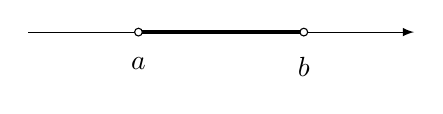
\begin{tikzpicture}[>=latex, scale=.7]
      \draw[->] (0.5,0)--(7.5,0);
      \draw[ultra thick] (2.5,0)node[below=5pt]{$a$}--(5.5,0)node[below=5pt]{$b$};
      \draw (2.5,0)[fill=white] circle (2pt);
      \draw (5.5,0)[fill=white] circle (2pt);
    \end{tikzpicture}
    \caption{}\label{fig:open_interval1}
  \end{minipage}
  \begin{minipage}[t]{0.48\textwidth}
    \centering
    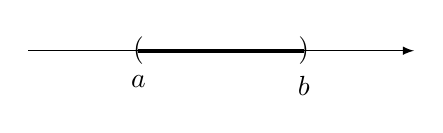
\begin{tikzpicture}[>=latex, scale=.7]
      \draw[->] (0.5,0)--(7.5,0);
      \draw[ultra thick] (2.5,0)node[below=5pt]{$a$}--(5.5,0)node[below=5pt]{$b$};
      \node at (2.5,0){$($}; \node at (5.5,0){$)$};
    \end{tikzpicture}
    \caption{}\label{fig:open_interval2}
  \end{minipage}
  \begin{minipage}[t]{0.48\textwidth}
    \centering
    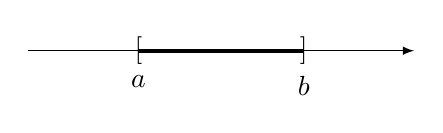
\begin{tikzpicture}[>=latex, scale=.7]
      \draw[->] (0.5,0)--(7.5,0);
      \draw[ultra thick] (2.5,0)node[below=5pt]{$a$}--(5.5,0)node[below=5pt]{$b$};
      \node at (2.5,0){$[$}; \node at (5.5,0){$]$};
    \end{tikzpicture}
    \caption{}\label{fig:close_interval}
  \end{minipage}
  \begin{minipage}[t]{0.48\textwidth}
    \centering
    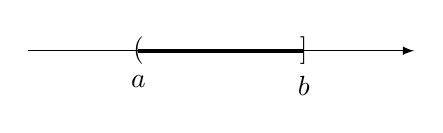
\begin{tikzpicture}[>=latex, scale=.7]
      \draw[->] (0.5,0)--(7.5,0);
      \draw[ultra thick] (2.5,0)node[below=5pt]{$a$}--(5.5,0)node[below=5pt]{$b$};
      \node at (2.5,0){$($}; \node at (5.5,0){$]$};
  \end{tikzpicture}
    \caption{}\label{fig:semi_open_interval1}
  \end{minipage}
  \begin{minipage}[t]{0.48\textwidth}
    \centering
    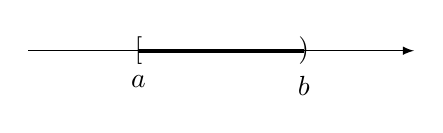
\begin{tikzpicture}[>=latex, scale=.7]
      \draw[->] (0.5,0)--(7.5,0);
      \draw[ultra thick] (2.5,0)node[below=5pt]{$a$}--(5.5,0)node[below=5pt]{$b$};
      \node at (2.5,0){$[$}; \node at (5.5,0){$)$};
    \end{tikzpicture}
    \caption{}\label{fig:semi_open_interval2}
  \end{minipage}
  \begin{minipage}[t]{0.48\textwidth}
    \centering
    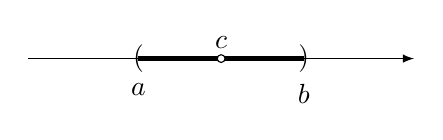
\begin{tikzpicture}[>=latex, scale=.7]
      \draw[->] (0.5,0)--(7.5,0);
      \draw[ultra thick] (2.5,0)node[below=5pt]{$a$}--(5.5,0)node[below=5pt]{$b$};
      \node at (2.5,0){$($}; \node at (5.5,0){$)$};
      \draw (4,0)[fill=white] circle (2pt)node[above]{$c$};
    \end{tikzpicture}
    \caption{}\label{fig:without_center_interval}
  \end{minipage}
\end{figure}

有时也要考虑无穷区间,用符号 $-\infty,+\infty$ 作为一端或两端,它们的记号和上面所引进的相类似,例如 $(-\infty,+\infty)$ 是全体实数集合 $\{x|x\in\mathbb{R}\}$, 区间 $(a,+\infty)$ 表示集合 $\{x|x>a\}$,区间 $(-\infty,b]$ 表示集合 $\{x|x\leqslant b\}$。无穷区间在几何上可用两端无限伸延的直线或一端无限伸延的射线来
表示。

以后我们要常用到一点的邻域的概念。\emph{$c$ 点的邻域}是包含 $c$ 点的任何开区间 $(a,b)$, 而 $c$ 点的去心邻域指去掉 $c$ 点的任何 $c$ 点的邻域。它的图象如\cref{fig:without_center_interval}。

$c$ 点的去心邻域可写成 $(a,c)\cup (c,b)$。我们常把 $c$ 点的邻域写成对称的形式:$(c-r,c+r)$,对任何 $r>0$, 并且称它为\emph{$c$ 点的对称邻域}。

\begin{example}
  试写出含于区间 $(1,5)$ 中 $\uppi$ 的对称邻域。
$\left(\uppi-\dfrac{1}{2},\uppi+\dfrac{1}{2}\right)$ 是含于 $(1,5)$ 的 $\uppi$ 对称邻域。此外 $(\uppi-1,\uppi+1)$,$\left(\uppi-\dfrac{3}{2},\uppi+\dfrac{3}{2}\right)$,$(\uppi-0.01,\uppi+0.01)$ 等都是含于 $(1,5)$ 中的对称邻域。
\end{example}

\subsection{函数的定义}
我们已经在第三册研究过许多函数,例如多项式函数、
三角函数,由于函数这个概念的重要性,并且它将是我们
的主要研究对象,因此需要回忆一般的函数的定义,下面我
们从数集之间的多对一(包括一对一)的关系重新给出函数
定义。

\begin{Definition}
设有数集 $A,B$,如果有一对应关系或法则 $f$ 存在,对于 $A$ 的任何一个数 $x$,有数集 $B$ 中唯一的一个数 $y$ 与之对应,我们就称给出了一个从数集 $A$ 到数集 $B$ 内的函数 $f$,用
\[f:A\mapsto B\]
表示,并写成 $y=f(x),\; (x\in A)$,此时称 $f(x)$ 为函数 $f$ 在 $x$ 的函数值,并称 $A$ 为函数 $f$ 的\emph{定义域}。又当 $x$ 取遍 $A$ 中的数时,函数值 $f(x)$ 全体也构成一个数集,称为函数 $f$ 的\emph{值域},记作
\[f(A)=\{f(x)|x\in A\}\]
要注意的是在构造一个函数 $f:A\mapsto B$ 的时候,$f(A)$ 不一定等
于 $B$, 而是 $B$ 的一个真子集,即 $f(A)\subset B$。
\end{Definition}



\begin{example}
设 $\mathbb{R}$ 是实数集,函数 $f:\mathbb{R}\mapsto\mathbb{R}$ 定义为
\[f(x)=\frac{2x}{x^2+1},\quad x\in(-\infty,+\infty)\]
求它的值域。
\end{example}

\begin{solution}
    方程 $f(x)=\dfrac{2x}{x^2+1}$ 等价于
    \begin{equation}
      \label{eq:function}
        yx^2-2x+y=0
    \end{equation}
根据函数的值域定义,任给 $y\in f(\mathbb{R})$, 方程 \eqref{eq:function} 必有实数
解,而方程 \eqref{eq:function} 有实数解的充要条件是
\[\Delta=1-y^2\geqslant 0\]
即:$-1\leqslant y\leqslant 1$,所以
\[f(\mathbb{R})=\{f(x)|-1\leqslant f(x)\leqslant 1\}\subset \mathbb{R}\]
\end{solution}

在函数的定义中包含三个要素,即\emph{定义域},\emph{多对一的对应法则}和\emph{函数值所在的数集}。应养成一个习惯,当给定一个函数时,必须指明它的定义域。在实际问题中,函数的定义域是根据实际意义来确定的,例如温度计刻有华氏温标度数 $F$ 和摄氏温标度数 $c$,因为不存在低于绝对零度的温度,因此,这两个度数之间的函数 $\varphi$ 是
\[F=\varphi(c)=\frac{9}{5}c+32,\quad c\in (-273,+\infty)\]

以后,当我们只在数学上,一般地研究一个具体解析式子规定的函数关系时,如果定义域$A$ 没有被指明,那么函数的定义域是使解析式子具有数值意义的所有 $x$ 的数值组成的
自然定义域,函数 $y$ 的值域通常是不指出的,因为由对应的规律本身就可以确定函数的值域。

\begin{example}
  求下列函数定义域:
\begin{tasks}(2)
  \task $f(x)=\dfrac{\sqrt{1-x}}{x}$
  \task $g(x)=\sqrt{x^2-1}$
\end{tasks}
\end{example}

\begin{solution}
    \begin{enumerate}
        \item \[\text{函数$f$有意义}\Leftrightarrow \begin{cases}
    1-x \geqslant 0\\
    x\ne 0
\end{cases}\Rightarrow\quad x\leqslant 1, \quad x\ne 0\]
$\therefore\quad $ 函数 $f$ 的定义域为 $(-\infty,0)\cup(0,1]$。

\item \[\text{函数$g$有意义}\Leftrightarrow x^2-1\geqslant 0 \Rightarrow\quad x\leqslant 1, \text{ 或 } x\geqslant 1\]
$\therefore\quad $ 函数 $g$ 的定义域为$(-\infty,-1]\cup[1,+\infty)$。
    \end{enumerate}
\end{solution}

\subsection{相等的函数}
怎样的两个函数是相等的函数?在数学中,有些函数可以用不同的方式来定义,例如,函数 $f:\mathbb{R}\mapsto \mathbb{R}^+\cup\{0\}$ 是由 $f(x)=|x|$ 规定的,而函数 $g:\mathbb{R}\mapsto \mathbb{R}^+\cup\{0\}$ 是由 $g(x)=\sqrt{x^2}$ 规定的,这里表示 $f(x)$ 与 $g(x)$ 的式子全不同,但是对于它们的相同的定义域中的任一 $x$ 值,经过不同规则的计算,它们的结果是相同的,即 $f(x)=g(x)$, 所以对于这个例子来说,尽管函数 $f(x),g(x)$ 的表达式不同,我们说 $f(x)$ 和 $g(x)$ 表示相同的函数。此外,解析式子相同,但定义域不同的函数是不相同的函数。例如:
\[\begin{split}
    f_1(x)&=\frac{1}{x},\qquad x\in (-\infty,0)\cup(0,+\infty)\\
    f_2(x)&=\frac{1}{x},\qquad x\in (0,+\infty)\\
    f_3(x)&=\frac{1}{x},\qquad x\in (0,1)
\end{split}\]
是不相同的函数,因为对于 $x=-2$, $f_1$ 有意义而 $f_2,f_3$ 都无
意义;对于 $x=2$, $f_1$ 和 $f_2$ 都有意义而 $f_3$ 无意义。

下面给出相等(同)的两个函数的条件。
\begin{Definition}{定义}
两个函数 $f:A\mapsto B$, $g:C\mapsto D$ 称为相等的当且仅当 $A=C$,$B=D$,且对于每个 $a\in  A$(或 $C$),有 $f(a)=g(a)$。
\end{Definition}

读者可能会不同意上面 $B=D$ 这个条件,提出下面这个例子来反驳:

“由 $f(n)=g(n)=n$ 给出的两个函数 $f:\mathbb{N}\mapsto\mathbb{N}$,$g: \mathbb{N}\mapsto \mathbb{Q}$ 是相等的函数”我们须指出两个函数不同的地方,就
函数值所在数集上看,$g$ 可以除以 2, 因此,对于 $g$ 我们可以构造一个新函数,
$\dfrac{1}{2}g:\mathbb{N}\mapsto \mathbb{Q}$, 这里
\[\left(\frac{1}{2}g\right)(n)=\frac{1}{2}n\]
但是对于 $f$, 不能做这种构造。

\subsection{函数的几个类型——满射、单射和双射}
现在,我们来讨论函数的三个重要类型,先给出定义,然后再举例说明。

\begin{Definition}
  如果在函数 $f:A\mapsto B$ 的 $B$ 中的每一个数 $b$ 在函数 $f$ 的作用下都是 $A$ 中一个数或某些数的对应数,也就是说:对于任意 $b\in B$,存在一个 $a\in A$,使得 $b=f(a)$,这样我们就说 $f$ 是由 $A$ 到 $B$ 的\emph{满射}。
\end{Definition}

显然,如果 $f:A\mapsto B$ 是满射,那么 $f(A)=B$。

第二类函数和满射同样地重要,叫做\emph{单射},定义如下:

\begin{Definition}
  如果对于 $A$ 中的任何两个不同的数 $a_1$ 和 $a_2$,就在 $B$ 中有两个不同的函数值 $f(a_1)$ 和 $f(a_2)$,即任何 $a_1,a_2\in A$,$a_1\ne a2\Rightarrow f(a_1)\ne f(a_2)$,那么我们就说 $f:A\mapsto B$ 是\emph{单射}(或一对一)。
\end{Definition}

 
它的逆否命题“如果在 $B$ 中有 $f(a_1)=f(a_2)$ 就在 $A$ 中有
$a_1=a_2$, 那么函数 $f:A\mapsto B$叫做\emph{单射}(或一对一)。”和上面
的定义等价,也常用来说明函数是一对一的。

还有一类很重要的函数叫做\emph{双射}。

\begin{Definition}
  函数 $f:A\mapsto B$,如果是满射又是单射,就叫做\emph{双射}。
\end{Definition}

\begin{example}
  函数 $f:\mathbb{R}\mapsto [-1,1]$,这里 $f(x)=\sin x, x\in\mathbb{R}$
是满射,但不是单射,因为对于 $\sin x=\dfrac{1}{2}\in [-1,1]$,
就有无穷多个 $x=\dfrac{\uppi}{6}+2k\uppi$ 或 $\dfrac{5\uppi}{6}+2k\uppi\;(k\in\mathbb{Z})$ 的值和它对应。
\end{example}

\begin{example}
  函数 $f:\mathbb{N}\mapsto\mathbb{N}$,这里 $f(n)=2n$ 是单射,但不是满射。
\end{example}

\begin{example}
  设 $2\mathbb{N}$ 代表偶数集,函数 $f:\mathbb{N}\mapsto 2\mathbb{N}$,这里$f(n)=2n$ 就是一双射。
\end{example}

\section{函数的运算与复合函数}

\subsection{函数的四则运算}

设 $f(x),g(x)$ 是两个 $x$ 的函数,它们的定义域分别为 $D_f$ 和 $D_g$,我们可以用通常对于“数”的四则运算得到它们的和函数 $(f+g)(x)$,差函数 $(f-g)(x)$,积函数 $(f\cdot g)(x)$ 与商函数 $\frac{f}{g}(x),\; g(x)\ne 0$。它们的定义域为 $D_f\cap D_g$。

由 $f(x),g(x)$ 的四则运算所得出来的新函数的定义如下:
\begin{itemize}[itemsep=7pt]
  \item $(f+g)(x)=f(x)+g(x)$ (即 $(f+g)$ 在 $x$ 点的值是 $f$,$g$ 的值的和);
  \item $(f-g)(x)=f(x)-g(x)$ (即 $(f-g)$ 在 $x$ 点的值是 $f$,$g$ 的值的差);
  \item $(f\cdot g)(x)=f(x)\cdot g(x)$ (即 $(f\cdot g)$ 在 $x$ 点的值是 $f$,$g$ 的值的积);
  \item $(f/g)(x)=f(x)/g(x)$ (即 $f/g$ 在 $x$ 点的值是 $f$,$g$ 的值的商,但只有在 $g(x)\ne 0$ 时才有意义)。
\end{itemize}

$f+g$, $f-g$ 和 $f\cdot g$ 的定义域是 $f$ 的定义域和 $g$ 的定义域的交集。而 $f/g$ 的定义域要从 $f$ 和 $g$ 的定义域的交集中去掉使 $g(x)=0$ 的值。

\begin{example}
  已知 $f(x)=\sqrt{x}$, $g(x)=\sqrt{1-x}$, 求 $f+g$,$f-g$,$f\cdot g$,$\dfrac{f}{g}$,$\dfrac{g}{f}$。
\end{example}

\begin{solution}
    $f$ 和 $g$ 的自然定义域是 $D_f=\{x|x\geqslant 0\}$, $D_g=\{x|x\leqslant 1\}$,$D_f$ 和 $D_g$ 的交集是 $D_f\cap D_g=[0,1]$。
\begin{itemize}[itemsep=7pt]
    \item 和:$(f+g)(x)=\sqrt{x}+\sqrt{1-x}$
    \item 差:$(f-g)(x)=\sqrt{x}-\sqrt{1-x}$
    \item 积:$(f\cdot g)(x)=\sqrt{x(1-x)}$
    \item 商:$\dfrac{f}{g}(x)=\sqrt{\dfrac{x}{1-x}},\qquad \dfrac{g}{f}(x)=\sqrt{\dfrac{1-x}{x}}$
\end{itemize}

$f+g$, $f-g$, $f\cdot g$ 的定义域是 $[0,1]$。因为当 $x=1$ 时,$g(x)=0$, 所以 $\dfrac{f}{g}$ 的定义域是 $[0,1)$, 同样得到 $\dfrac{g}{f}$ 的定义域 $(0,1]$。
\end{solution}

\begin{example}
设$f(x)=\sin x$, $g(x)=\cos x$,$D_f=(-\infty,+\infty)$,$D_g=(-\infty,+\infty)$,则:
\[\begin{split}
    (f+g)(x)=\sin x+\cos x&=\sqrt{2}\left(\frac{1}{\sqrt{2}}\sin x+\frac{1}{\sqrt{2}}\cos x\right)\\
    &=\sqrt{2}\left(\sin x\cos\frac{\uppi}{4}+\cos x\sin\frac{\uppi}{4} \right)\\
    &=\sqrt{2}\sin\left(x+\frac{\uppi}{4}\right)\\
    (f-g)(x)=\sin x-\cos x&=\sqrt{2}\sin\left(x-\frac{\uppi}{4}\right)\\
    (f\cdot g)(x)=\sin x\cdot \cos x&=\frac{1}{2}\sin 2x\\
    \left(\frac{f}{g}\right)(x)=\frac{\sin x}{\cos x}&=\tan x\\
\end{split}\]    

这里 $f+g$, $f-g$, $f\cdot g$ 的定义域是 $(-\infty,+\infty)$,$\dfrac{f}{g}$ 的定义域是
\[\left\{x\big|x\in\mathbb{R},\; x\ne \frac{\uppi}{2}+k\uppi,\; k\in \mathbb{Z}\right\}\]
\end{example}

\subsection{复合函数}
上面我们是用四则运算来组合已知函数为一个新函数的,但是构成新的函数的方法,还有一个更重要的运算叫做组成函数的函数或复合函数法。

我们先从一个简单的例子说起,火箭从地面上的 $L$ 点垂直向上发射,火箭 $R$ 在 $t$ 秒后离开发射点的距离是 $h(t)$, 这个函数是已知的。在离发射座 \qty{1}{km} 远的地方有一个观测站 $O$,我们要求把火箭与观测站的距离 $d$ 确定为时间 $t$ 的函数(\cref{fig:function_d_vs_t})。
\begin{figure}
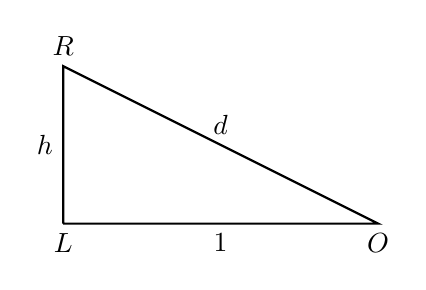
\begin{tikzpicture}[thick]
\draw (0,0)node[below]{$L$}--node[below]{1}(4,0)node[below]{$O$}--node[above]{$d$}(0,2.0)node[above]{$R$}--node[left]{$h$}(0,0);
\end{tikzpicture}
    \caption{}\label{fig:function_d_vs_t}
\end{figure}

我们已经知道火箭的垂直高度 $h$ 是 $t$ 的函数 $h(t)$,又火箭到观测站的距离 $d$ 又是火箭的高度 $h$ 的函数
\[d=\sqrt{1+h^2}\]
因此在时刻 $t$,$R$ 到 $O$ 的距离是
\[d(t)=\sqrt{1+h^2(t)}\]

上面函数 $d(t)$ 是由 $h=h(t)$ 和 $d=f(h)=\sqrt{1+h^2}$ 两个函数构成的,把其中一个函数 $h(t)$ 代入另一个函数 $f(h)$ 的运算叫做复合运算,得到的函数 $d(t)=f\big(h(t)\big)$ 叫做 $t$ 的复合函数。

一般说来,若 $z=f(y)$, $y=g(x)$,且 $g(x)$ 的值域含于 $f(y)$ 的定义域中,那么对于 $g(x)$ 定义域内的每一个 $x$ 值经过中间变数 $y$,相应地得到唯一确定的一个值$z$,变数 $z$ 经过中间变数 $y$ 而成变数 $x$ 的函数,记为 $z=f\big(g(x)\big)$,这个函数称为前两个函数的\emph{复合函数}。应该指出,函数 $y=g(x)$ 的值域不能超出函数 $f(y)$ 的定义域,这是极重要的。


\begin{example}
    设 $z=\sqrt{1+y}$, 它的定义域 $D_y=[-1,+\infty)$,再设 $y=x^2-5$,它的定义域 $D_x=(-\infty,+\infty)$, 值域 $R=[-5,+\infty)$。

作为复合函数 $z=\sqrt{1+(x^2-5)}=\sqrt{x^2-4}$,其定义域只能是 $(-\infty,-2]$ 和$[2,+\infty)$,这时,$y=x^2-5$ 的值域是 $[-1,+\infty)$, 它没有超过 $D_y=[-1,+\infty)$ 的范围,这就是说复合函数 $z=f\big(g(x)\big)$ 的定义域只能由 $y=
g(x)$ 的定义域中那些使 $g(x)$ 属于 $z=f(y)$ 的定义域的 $x$ 组成。
\end{example}

\begin{example}
已知 $f(g)=\dfrac{1}{g+1}$,$g=g(x)=x^2$。

求 $f\big(g(x)\big)$ 和 $g\big(f(x)\big)$。    
\end{example}

\begin{solution}
\[\begin{split}
    f\big(g(x)\big)&=\frac{1}{x^2+1}\\
    g\big(f(x)\big)&=\left(\frac{1}{x+1}\right)^2=\frac{1}{x^2+2x+1}
\end{split}\]
显然,$f\big(g(x)\big)\ne g\big(f(x)\big)$, 这表明函数的复合运算是不满足交换律的。
\end{solution}

\begin{example}
已知 $f\left(\sin\dfrac{x}{2}\right)=\cos x+1$,
求 $f\left(\cos\dfrac{x}{2}\right)$。
\end{example}    

\begin{solution}
复合函数 $f\left(\sin\dfrac{x}{2}\right)=\cos x+1=2-2\sin^2\dfrac{x}{2}$ 是把函数 $y=\sin\frac{x}{2}$ 代入 $f(y)=2-2y^2$ 中复合而成。现在令 $y=\cos\dfrac{x}{2}$ 代入 $f(y)$,得到
\[f\left(\cos\frac{x}{2}\right)=2-2\cos^2\frac{x}{2}=2-(1+\cos x)=1-\cos x\]
\end{solution}    

在函数的运算中,我们介绍了函数的加、减、乘、除和函数的复合五种运算,从定义来看,我们可以用上述五种运算,由某一简单而基本的函数去造出多种多样的新函数来,譬如从常数函数 $y=c$ 和恒等函数 $y=x$,用加、减、乘运算就可以得出多项式函数。其实我们常常要用到的,并不是把所给的函数组合成更复杂的函数;而是要把所给的函数分解成更简
单的函数的组合,把要解的问题归于比较简单的问题去解决。

\begin{example}
    将函数 $y=x\sin\dfrac{1}{x}$ 分解成比较简单的函数的组合(引进新的中间变数符号)。
\end{example}

\begin{solution}
$y=x\sin\dfrac{1}{x}$ 可分解为 $f(x)=x$ 与 $g(x)=\sin\dfrac{1}{x}$ 之积,又$g(x)=\sin\dfrac{1}{x}$ 可以看作是 $g(h)=\sin h$ 和 $h=h(x)=\dfrac{1}{x}$ 的复合函数,于是原来的函数可以看作下面简单函数的组合
\[F(x)=f(x)\cdot g\big(h(x)\big)\]
这里 $f(x)=x$,$g(h)=\sin h$,$h=h(x)=\dfrac{1}{x}$。    
\end{solution}

\begin{example}
求函数 $\sqrt{x-\sqrt{x+1}-2}$ 的定义域。
\end{example}

\begin{solution}
设 $F(x)=\sqrt{x-\sqrt{x+1}-2}=\sqrt{(x+1)-\sqrt{x+1}-3}$,则 $F(x)$ 可以看作$f(y)=\sqrt{y^2-y-3}$ 与 $y=g(x)=\sqrt{x+1}$ 的复合函数,即$F(x)=f\big(g(x)\big)$ 且知:

$f(y)$ 的定义域 $D_f=\left(-\infty,\dfrac{1-\sqrt{13}}{2}\right]\bigcup\left[\dfrac{1+\sqrt{13}}{2},+\infty\right)$

$g(x)$ 的定义域 $D_g=[-1,+\infty)$, 它的值域$R_x=[0,+\infty)$

\[\begin{split}
&\text{复合函数 $F(x)=f\big(g(x)\big)$有意义}\Longleftrightarrow
\begin{cases}
    g(x)\text{有意义}\\
    g(x)\in\left[\dfrac{1+\sqrt{13}}{2},+\infty\right)
\end{cases}\\
&\Longleftrightarrow
\begin{cases}
    x+1\geqslant 0\\
    \sqrt{x+1}\geqslant \dfrac{1+\sqrt{13}}{2}
\end{cases}\Longleftrightarrow
\begin{cases}
    x\geqslant -1\\
    x+1\geqslant \left(\dfrac{1+\sqrt{13}}{2}\right)^2=\dfrac{7+\sqrt{13}}{2}
\end{cases}\\
&\Longleftrightarrow x\geqslant \frac{5+\sqrt{13}}{2}
\end{split}\]
$\therefore\quad $ 函数 $\sqrt{x-\sqrt{x+1}-2}$ 的定义域是
$\left[\dfrac{5+\sqrt{13}}{2},+\infty\right)$。

如果直接求$F(x)=\sqrt{x-\sqrt{x+1}-2}$的定义域,那
么只须:
\[\begin{split}
   x-\sqrt{x+1}-2\geqslant 0& \Longleftrightarrow x-2\geqslant \sqrt{x+1} \Longleftrightarrow \begin{cases}
    x-2\geqslant 0\\ x+1\geqslant 0\\ (x-2)^2\geqslant (x+1)
\end{cases}\\
& \Longleftrightarrow \begin{cases}
    x\geqslant 2\\x\geqslant -1\\ x\geqslant \dfrac{5+\sqrt{13}}{2}
\end{cases} \Longleftrightarrow x\geqslant \frac{5+\sqrt{13}}{2}
\end{split}\]
$\therefore\quad $ 函数 $\sqrt{x-\sqrt{x+1}-2}$ 的定义域是
$\left[\dfrac{5+\sqrt{13}}{2},+\infty\right)$。
\end{solution}

\begin{Exercise}

\begin{question}
  \item 试确定下面每一对函数 $f$ 和 $g$ 的自然定义域,并求 $f+g$, $f-g$, $f\cdot g$, $f/g$ 和 $g/f$ 的相应的定义域。
  \begin{tasks}(2)
    \task $f(x)=x,\qquad g(x)=\sqrt{x-1}$
    \task $f(x)=\frac{1}{x-2},\qquad g(x)=\frac{1}{\sqrt{x-1}}$
    \task $f(x)=\sqrt{x},\qquad g(x)=\sqrt[4]{x+1}$
    \task $f(x)=\sin x,\qquad g(x)=\cos x$
    \task $f(x)=\tan x,\qquad g(x)=\tan x$
  \end{tasks}
    \item 证明函数 $f(x)=\dfrac{1}{1+x}$ 在它的定义域上是单射的。又 $x$ 为何值时,下列各式才有意义?
\begin{tasks}(2)
    \task $f\big(f(x)\big)$
    \task $f\left(\dfrac{1}{x}\right)$
    \task $f(cx)$
    \task! 对于哪些数 $c$,有一数 $x$ 能使 $f(cx)=f(x)$
\end{tasks}        

\item 下列函数能否构成复合函数 $y=f\big(\varphi(x)\big)$,如果能够
构成,则指出复合函数的定义域和值域:
\begin{tasks}
    \task $y=f(u)=2u+1,\qquad u=\varphi(x)=x^2$
    \task $y=f(u)=\sqrt{u},\qquad u=\varphi(x)=1-x^2$
    \task $y=f(u)=u^2+u^3, \qquad u=\varphi(x)=\begin{cases}
        1,& \text{当 $x$ 为有理数}\\
        2,&\text{当 $x$ 为无理数}\\
    \end{cases}$
    \task $y=f(u)=2$,定义域为 $U_1$,\qquad  $u=\varphi(x)$,定义域为 $X$,值域为 $U_2$。
\end{tasks}

\item 设$f(x)=ax^2+bx+c$,证明
$f(x+3)-3f(x+2)+3f(x+1)-f(x)=0$。
\item 
\begin{tasks}
\task 设 $y=f(x)=a+bx+\dfrac{c}{x}$,求 $f\left(\dfrac{2}{x}\right)$。
\task 设 $y=f(x)=\sqrt{1+x+x^2}$,求 $f(x^2)$, $f(-x^2)$。
\end{tasks}

\item 若 $\varphi(x)=x^3+1$,求 $\varphi(x^2)$,$\big(\varphi(x)\big)^2$, $\varphi\big(\varphi(x)\big)$。
\item 求下列函数定义域:
 \begin{tasks}(2)
    \task $y=\sqrt{x}+\sqrt{-x}$
    \task $y=\sqrt[\uproot{10}\leftroot{-3}4]{\dfrac{(x-2)(x-3)}{x^2}}$
\end{tasks}   

\item $a,b,c,d$ 取什么值,才能使函数
\[f(x)=\frac{ax+b}{cx+d}\]
对所有 $x$ 满足 $f\big(f(x)\big)=x$?
\end{question}
\end{Exercise}

\section{函数的图象}

从平面上一条曲线(对这条曲线应该要求:与纵轴平行的直线与它的交点不能多于一个)可以引出一个函数,反过来,给了一个函数 $y=f(x)$, 那么通常采用直角坐标系,就可以用图形来表示 $y$ 是 $x$ 的函数。

定义在某一变域 $D$ 上的函数的图象就是让 $x$ 取遍 $D$ 中所有值,所有点 $(x,f(x))$ 的集合便形成平面上的一个\emph{图形},这个图形称为函数 $y=f(x)$的\emph{图象},而这个方程 $y=f(x)$ 称为\emph{图象的方程}。

利用函数图象的几何直观可以更清楚地看出函数的一些性质,下面我们把函数的解析性质和它的图象上相应的几何性质对照着列出来:

% \begin{table}
\medskip\noindent{\small
\begin{tblr}{colspec={cX[l]X[l]},hline{2}=0.8pt}
  &  解析性质  & 几何性质 \\
1 & $f$ 是 $x$ 的增函数,即对于任意的 $a\in D$,$b\in D$,当 $a<b$ 时,恒有 $f(a)<f(b)$  & $f$ 的图象随着 $x$ 向右移动而上升\\
2 & $f$ 是 $x$ 的减函数,即对于任意的$a\in D$,$b\in D$,当 $a<b$ 时,恒有 $f(a)>f(b)$ & $f$ 的图象随着向右移动而下降\\
3 & $f$ 是偶函数,即对于任意的 $x\in D$,恒有 $f(-x)=f(x)$  & 函数 $f$ 的图象关于 $y$ 轴对称\\
4 & $f$ 是奇函数,即对于任意的 $x\in D$,恒有 $f(-x)=-f(x)$ & 函数 $f$ 的图象关于原点对称\\
5 & $f$ 是周期函数,即对于任意的 $x\in\mathbb{R}$,恒有 $f(x+p)=f(x)$,这里 $p$ 是一个正的常数 & 函数 $f$ 在区间 $[0,p]$ 或 $\left[-\dfrac{p}{2},\dfrac{p}{2}\right]$ 上的
图象可以沿 $x$ 轴左、右连续推移,重复出现\\
\end{tblr}}
% \end{table}

\medskip 下面我们给出几个常见的函数的图象。

\subsubsection{常值函数}
常值函数 $f(x)=c$ 的图象是一条平行 $x$ 轴的直线,它至 $x$ 轴的距离为 $|c|$, 如\cref{fig:function_const}。

\subsubsection{取整函数}
函数 $f(x)=[x]$ 代表不超过 $x$ 的最大整数,即:若 $n\leqslant x<n+1,\; n\in\mathbb{Z}$,则$f(x)=[x]=n$。它的图象如\cref{fig:function_sign}。

\begin{figure}
  \begin{minipage}[t]{0.48\textwidth}
    \centering
    \begin{tikzpicture}[>=latex, scale=0.85]
      \draw[->] (-2.5,0)--(2.5,0)node[right]{$x$};
      \draw[->] (0,-1)--(0,2.5)node[right]{$y$};
      \draw[very thick] (-2,1.5)--(2,1.5)node[above]{$f(x)=c$};
      \draw[<->] (-1,0)--node[right]{$c$}(-1,1.5);
      \node at (-.25,-.25){$O$};
    \end{tikzpicture}
    \caption{}\label{fig:function_const}
  \end{minipage}
  \begin{minipage}[t]{0.48\textwidth}
    \centering
    \begin{tikzpicture}[>=latex, scale=0.85]
      \draw[->] (-2.5,0)--(3.5,0)node[right]{$x$};
      \draw[->] (0,-2.5)--(0,2.5)node[right]{$y$};
      \foreach \x in {-2,-1,1,2,3}
      {
          \draw (\x,0)node[below]{$\x$}--(\x,.1);
      }     
      \foreach \x in {1,2}
      {
          \draw (0,\x)node[left]{$\x$}--(.1,\x);
      }
      \foreach \x in {-1,-2}
      {
          \draw (0,\x)--(.1,\x)node[right]{$\x$};
      }
      \foreach \x in {-2,-1,...,2}
      {
          \draw [very thick](\x,\x)--(\x+1,\x);
          \draw (\x+1,\x)[fill=white] circle(1.5pt);
      }
      \node at (-.25,-.25){$O$};
    \end{tikzpicture}
    \caption{}\label{fig:function_sign}
  \end{minipage}
\end{figure}

\subsubsection{一次函数}

我们已经在第三册中知道,一次函数 $f(x)=kx+b\; (k\ne 0)$ 的图象是不平行于 $x$ 轴和 $y$ 轴的直线。$k$ 称为直线的斜率,$b$ 称为直线的 $y$ 截距。若知一次函数图象上的两个点,我们用直线方程的两点式:
\[y-y_1=\frac{y_2-y_1}{x_2-x_1}(x-x_1)\]
就可以写出一次函数的关系式。

下面给出的函数的图象是有间断点的直线:
\begin{figure}
  \begin{tikzpicture}[>=latex, scale=1]
    \draw[->] (-2.5,0)--(3,0)node[right]{$x$};
    \draw[->] (0,-1)--(0,2.5)node[right]{$y$};
    \foreach \x in {-1,1}
    {
        \draw (\x,0)node[below]{$\x$}--(\x,.1);
    }
    \draw[domain=-2:2, samples=10, very thick]plot(\x, {0.75*(\x+1)});
    \draw[dashed] (0,1.5)node[left]{$1\dfrac{1}{2}$}--(1,1.5)--(1,0);
    \draw (1,1.5) [fill=white] circle(1.5pt)node[right]{$\left(1,1\dfrac{1}{2}\right)$};
    \node at (2,2)[above]{$y=\dfrac{3}{4}(x+1)$};
    \node at (.25,-.25){$O$};
  \end{tikzpicture}    
  \caption{}\label{fig:function_linear}
\end{figure}

函数 $f(x)=\dfrac{3}{4}\cdot \dfrac{x^2-1}{x-1}$,$x\in (-\infty,1)\cup(1,+\infty)$ 的图象是一条有间断点 $\left(1,1\dfrac{1}{2}\right)$ 的直线,除去点 $\left(1,1\dfrac{1}{2}\right)$ 外,它与直线 $y=\dfrac{3}{4}(x+1)$一致。(见\cref{fig:function_linear})

\subsubsection{阶梯函数}
设点列 $\{x_i\},\; i=0,1,\ldots,n$ 是闭区间 $[a,b]$ 中的递增点列,使得 $x_0=a$, $x_n=b$,即 $a=x_0<x_1<x_2<\cdots<x_{n-1}<x_n=b$,且当 $x_{i-1}<x<x_i$ 时,$f(x)=k_i,\; i=1,2,\ldots,n$。而 $x$ 在分点,$x_i,\; i=0,1,\ldots,n$ 的值 $f(x_i)$ 可以任意给定,这样一个在 $[a,b]$ 上有定义的,而在每个子区间 $(x_{i-1},x_i),\; i=1,2,\ldots,n$ 都是常数的函数叫做阶梯函数。

例如,定义在 $[0,6]$ 上的阶梯函数 $f$:
\[\begin{cases}
   f(0)=2.5,\\
f(x)=2 ,&0<x\leqslant 1,\\
f(x)=0,&1<x\leqslant 2,\\
f(x)=-1,&2<x\leqslant 4,\\
f(x)=2 ,&4<x\leqslant 6. \\
\end{cases}\]
的图象如\cref{fig:function_step} 所示。

\begin{figure}[htp]\centering
    \begin{minipage}[t]{0.48\textwidth}
    \centering
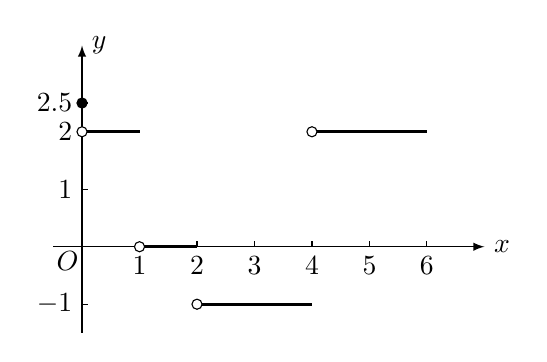
\begin{tikzpicture}[>=latex, scale=.73]
    \draw[->] (-.5,0)--(7,0)node[right]{$x$};
    \draw[->] (0,-1.5)--(0,3.5)node[right]{$y$};
\foreach \x in {1,2,...,6}
{
\draw (\x,0)node[below]{$\x$}--(\x,.1);
}
\node at (-.25,-.25){$O$};
\foreach \x in {-1,1,2,2.5}
{
\draw (0,\x)node[left]{$\x$}--(.1,\x);
}

\draw[very thick] (0,2)--(1,2);
\draw[very thick] (1,0)--(2,0);
\draw[very thick] (2,-1)--(4,-1);
\draw[very thick] (4,2)--(6,2);
\foreach \x in {{0,2},{1,0},{2,-1},{4,2}}
{
\draw (\x)[fill=white] circle(2.5pt);
}
\draw (0,2.5)[fill=black] circle(2.5pt);
    \end{tikzpicture}
    \caption{}\label{fig:function_step} 
    \end{minipage}
    \begin{minipage}[t]{0.48\textwidth}
    \centering
    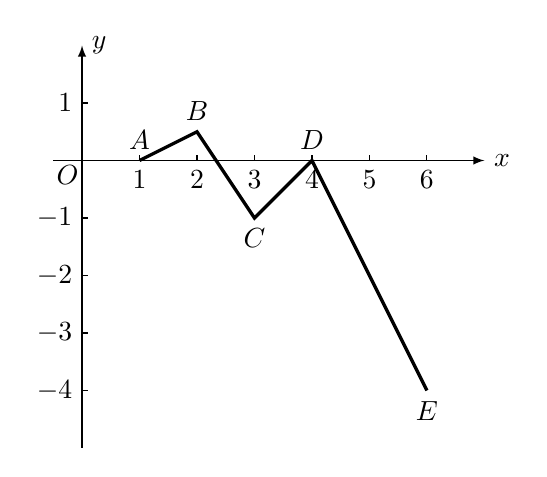
\begin{tikzpicture}[>=latex, scale=.73]
        \draw[->] (-.5,0)--(7,0)node[right]{$x$};
        \draw[->] (0,-5)--(0,2)node[right]{$y$};
\foreach \x in {1,2,...,6}
{
    \draw (\x,0)node[below]{$\x$}--(\x,.1);
}
\node at (-.25,-.25){$O$};
\foreach \x in {1,-1,-2,...,-4}
{
    \draw (0,\x)node[left]{$\x$}--(.1,\x);
}

\draw[very thick] (1,0)node[above]{$A$}--(2,.5)node[above]{$B$}--(3,-1)node[below]{$C$}--(4,0)node[above]{$D$}--(6,-4)node[below]{$E$};

    \end{tikzpicture}
    \caption{}\label{fig:function_multiline} 
    \end{minipage}
    \end{figure}

\subsubsection{折线函数}
我们定义 $g$:
\[g(x)=\begin{cases}
    \dfrac{1}{2}(x-1), & x\in[1,2]\\
    -\dfrac{3}{2}(x-2)+\dfrac{1}{2}(2-1),& x\in [2,3]\\
    (x-3)-\dfrac{3}{2}(3-2)+\dfrac{1}{2}(2-1),& x\in [3,4]\\
  -2(x-4)+(4-3)-\dfrac{3}{2}(3-2)+\dfrac{1}{2}(2-1),& x\in [4,6]\\
\end{cases}\]
它的图象是一条折线 $ABCDE$, 如\cref{fig:function_multiline} 。


\subsubsection{幂函数}
函数 $f(x)=x^n$,其中 $n$ 为任意自然数,称为正整指数幂函数。

为了了解正整指数幂函数的一般性质,我们在同一个坐标系内,绘出几个这样的函数,如\cref{fig:function_power}。
\begin{figure}
  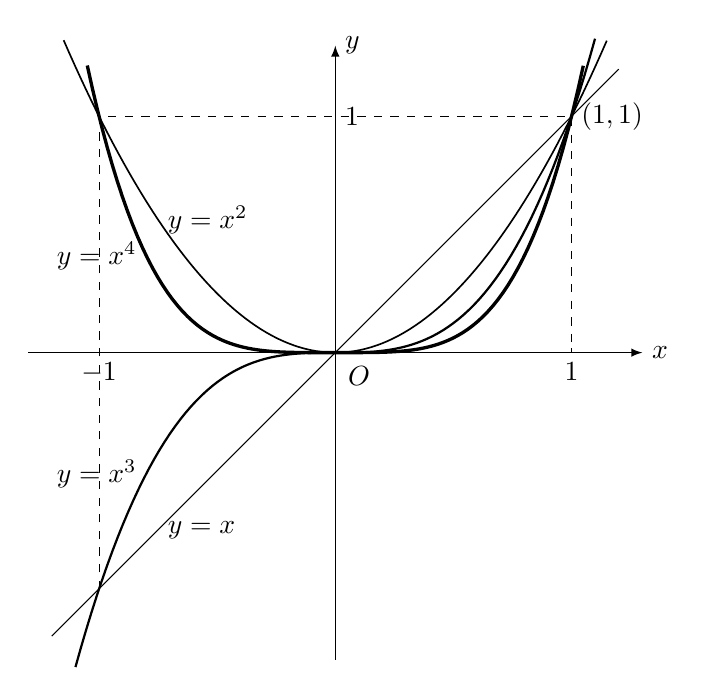
\begin{tikzpicture}[>=latex, scale=3]
    \draw[->] (-1.3,0)--(1.3,0)node[right]{$x$};
    \draw[->] (0,-1.3)--(0,1.3)node[right]{$y$};
    \foreach \x in {-1,1}
    {
        \draw (\x,0)node[below]{$\x$}--(\x,.02);
    }
    \node at (.1,-.1){$O$};
    \draw[dashed](-1,-1)--(-1,1)--(1,1)--(1,0);
    \draw (-1.2,-1.2)--(1.2,1.2);
    \draw [domain=-1.15:1.15, samples=100, semithick]plot(\x, {\x*\x});
    \draw [domain=-1.1:1.1, samples=100, thick]plot(\x, {\x*\x*\x});
    \draw [domain=-1.05:1.05, samples=100, very thick]plot(\x, {\x*\x*\x*\x});
    \node at (0,1)[right]{1};
    \node at (1,1)[right]{$(1,1)$};
    \node at (-.75,-.75)[right]{$y=x$};
    \node at (-.8,-.512)[left]{$y=x^3$};
    \node at (-.75,.5625)[right]{$y=x^2$};
    \node at (-.8,.41)[left]{$y=x^4$};
  \end{tikzpicture}    
  \caption{}\label{fig:function_power}
\end{figure}

显然,当 $n$ 为奇数时,因为 $f(-x)=(-x)^n=-x^n=-f(x)$,所以函数是奇函数。又所有正整指数幂函数,当 $x=0$ 时,$f(0)=0$。故每个奇次幂函数的图象通过原点,位于第一和第三象限内且关于原点对称。所有这样的函数都是增函数。

当 $n$ 为偶数时,因为 $f(-x)=(-x)^n=x^n=f(x)$,所以函数是偶函数,每个图象通过原点,位于第一和第二象限内且关于 $y$ 轴对称。

由于当 $x=1$ 时,$f(1)=1^n=1$, 每个正整指数幂函数的图象都通过点 $(1,1)$。

现在让指数 $n$ 逐次增大,看看图象的变化,从\cref{fig:function_evenpower,fig:function_oddpower} 可以清楚地看出每个图象的平坦部分和陡峭部分,曲线最终以\cref{fig:function_evenpower,fig:function_oddpower} 中的粗黑线为极限位置。

\begin{figure}
  \begin{minipage}[t]{0.48\textwidth}
  \centering
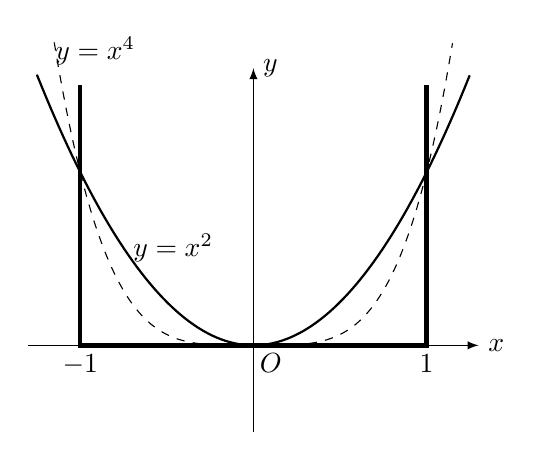
\begin{tikzpicture}[>=latex, scale=2.2]
  \draw[->] (-1.3,0)--(1.3,0)node[right]{$x$};
  \draw[->] (0,-.5)--(0,1.6)node[right]{$y$};
\foreach \x in {-1,1}
{
\draw (\x,0)node[below]{$\x$}--(\x,.02);
}
\node at (.1,-.1){$O$};
\draw[ultra thick](-1,1.5)--(-1,0)--(1,0)--(1,1.5);
\draw [domain=-1.25:1.25, samples=100, thick]plot(\x, {\x*\x});
\draw [domain=-1.15:1.15, samples=100, dashed]plot(\x, {\x*\x*\x*\x});
\node at (-.75,.5625)[right]{$y=x^2$};
\node at (-1.2,1.7)[right]{$y=x^4$};      
  \end{tikzpicture}
  \caption{}\label{fig:function_evenpower}
  \end{minipage}
  \begin{minipage}[t]{0.48\textwidth}
  \centering
  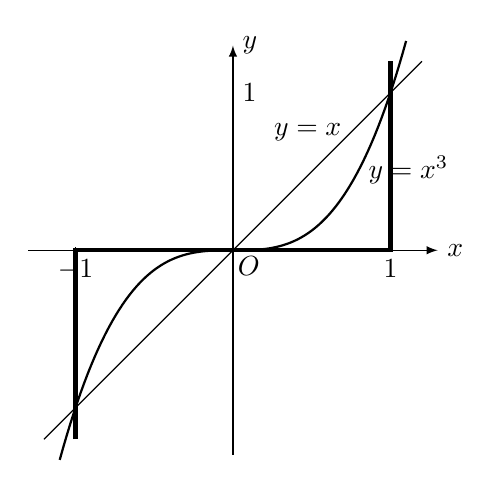
\begin{tikzpicture}[>=latex, scale=2]
      \draw[->] (-1.3,0)--(1.3,0)node[right]{$x$};
      \draw[->] (0,-1.3)--(0,1.3)node[right]{$y$};
\foreach \x in {-1,1}
{
  \draw (\x,0)node[below]{$\x$}--(\x,.02);
}
\node at (.1,-.1){$O$};
\draw[ultra thick](-1,-1.2)--(-1,0)--(1,0)--(1,1.2);
\draw (-1.2,-1.2)--(1.2,1.2);
\draw [domain=-1.1:1.1, samples=100, thick]plot(\x, {\x*\x*\x});
\node at (0,1)[right]{1};
\node at (.75,.75)[left]{$y=x$};
\node at (.8,.512)[right]{$y=x^3$};
  \end{tikzpicture}
  \caption{}\label{fig:function_oddpower}
  \end{minipage}
  \end{figure}

函数 $f(x)=x^{-n}$($x\ne 0$, $n$ 为自然数)称为负整指数幂函数。在同一坐标系内,绘出 $y=x^{-1}$, $y=x^{-2}$, $y=x^{-3}$, $y=x^{-4}$ 的图象如\cref{fig:function_negative_power} 所示。当 $x=0$ 时,这些函数都无意义,函数的图象在此点断开,它的二支以 $y$ 轴为渐近线。

当指数为负奇数时,这些函数是奇函数。图象的二支分别位于第一和第三象限内,随 $x$ 向右移动下降,且关于原点对称。因此,函数在 $(-\infty,0)$ 或 $(0,+\infty)$ 内是减函数。

当指数是负偶数时,这些函数是偶函数,每个函数的图象在原点处断开,分为二支,位于第一和第二象限内,都以 $y$ 轴为渐近线,且关于 $y$ 轴对称。从图象明显地看出,当 $x<0$ 时,函数是增函数,当 $x>0$ 时,函数是减函数。

\begin{figure}
  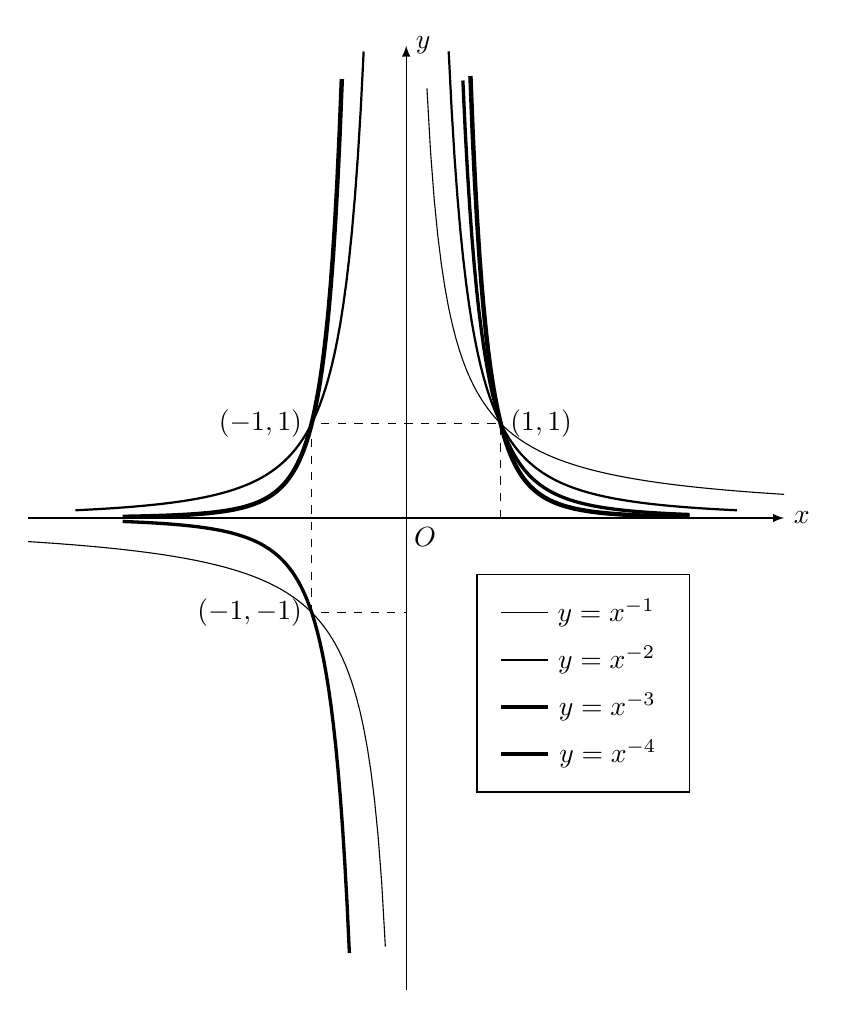
\begin{tikzpicture}[>=latex, scale=1.2]
      \draw[->] (-4,0)--(4,0)node[right]{$x$};
      \draw[->] (0,-5)--(0,5)node[right]{$y$};
  \draw [domain=-4:-.22, samples=100]plot(\x, {1/\x});
  \draw [domain=-3.5:-.45, samples=100, thick]plot(\x, {1/(\x*\x)});
  \draw [domain=-3:-.6, samples=100, very thick]plot(\x, {1/(\x*\x*\x)});
  \draw [domain=-3:-.68, samples=100, ultra thick]plot(\x, {1/(\x*\x*\x*\x)});  
  \node at (.2,-.2){$O$};
  \draw [domain=.22:4, samples=100]plot(\x, {1/\x});
  \draw [domain=.45:3.5, samples=100, thick]plot(\x, {1/(\x*\x)});
  \draw [domain=.6:3, samples=100, very thick]plot(\x, {1/(\x*\x*\x)});
  \draw [domain=.68:3, samples=100, ultra thick]plot(\x, {1/(\x*\x*\x*\x)});  
  \draw[dashed](1,0)--(1,1)node[right]{$(1,1)$}--(-1,1)node[left]{$(-1,1)$}--(-1,-1)node[left]{$(-1,-1)$}--(0,-1);
  \draw (1,-1)--(1.5,-1)node[right]{$y=x^{-1}$};
  \draw[thick] (1,-1.5)--(1.5,-1.5)node[right]{$y=x^{-2}$};
  \draw[very thick]  (1,-2)--(1.5,-2)node[right]{$y=x^{-3}$};
  \draw[ultra thick]  (1,-2.5)--(1.5,-2.5)node[right]{$y=x^{-4}$};
  \draw (.75,-.6) rectangle (3,-2.9);
  \end{tikzpicture}
      \caption{}\label{fig:function_negative_power}
  \end{figure}

下面我们来说明一些函数的图象如何由另一些函数的已知图象经过某些几何变换得到。

若对于任意的 $x\in D$, 函数 $f$ 和 $g$ 满足 $g(x)=f(x-c)$,这里 $c$ 是常数,则若 $c>0\; (c<0)$,$y=g(x)$ 的图象可以由 $y=f(x)$ 的图象,平行 $x$ 轴右移(或左移) $|c|$ 个单位得到。

若函数 $f$ 和 $g$ 满足等式 $g(x)=f(kx)$,这里 $k$ 是常数,则若 $k>1\; (0<k<1)$, $y=g(x)$ 的图象可以由 $y=f(x)$ 的图象经过把它上面的所有点的横坐标垂直于 $y$ 轴压缩(或拉长)$k$ 倍而纵坐标不变的几何变换得到。

若函数 $f$ 和 $g$ 满足等式,$g(x)=kf(x)$,这里 $k$ 是常数,则若 $k>1\; (0<k<1)$,$y=g(x)$ 的图象可以由 $y=f(x)$ 的图象经过把它上面的所有点的纵坐标垂直 $x$ 轴拉长(或压缩)$k$ 倍而使横坐标不变的几何变换得到。

下面我们用例子说明图象的几何变换。

\begin{example}
  说明 $y=f(x)=\sin x$ 和 $y=g(x)=\cos x$ 的图象的关系。
\end{example}

\begin{solution}
这两个函数的定义域都是 $(-\infty,+\infty)$,根据 $f(x)=\sin x$ 和 $g(x)=\cos x$ 是周期等于 $2\uppi$ 的函数,因此我们可以先在长度等于 $2\uppi$ 的区间上来讨论这两个函数。

{\linespread{2.0}\selectfont
设 $f(x)=\sin x$ 的定义域 $D_y=[0,2\uppi]$,因为余弦函数 $g(x)=\cos x$ 可以看作正弦函数 $\sin x$ 与 $x'=x+\dfrac{\uppi}{2}$ 的复合函数,即 $g(x)=\cos x=\sin\left(x+\dfrac{\uppi}{2}\right)$,所以复合函数 $\sin\left(x+\dfrac{\uppi}{2} \right)$ 有意义,必须且只须 $0\leqslant x+\dfrac{\uppi}{2}\leqslant 2\uppi$,由此得到 $-\dfrac{\uppi}{2}\leqslant x\leqslant \dfrac{3\uppi}{2}$。

这就是说 $y=g(x)=\cos x$ 的定义域是 $D_g=\left[-\dfrac{\uppi}{2},\dfrac{3\uppi}{2}\right]$。因为区间 $D_g$ 是把区间 $D_f$ 左移了 $\dfrac{\uppi}{2}$ 个单位的结果,并且对于 $D_g=\left[-\dfrac{\uppi}{2},\dfrac{3\uppi}{2}\right]$ 中的每一个 $x$ 都可以在 $D_f=[0,2\uppi ]$ 中找到相应的 $x+\dfrac{\uppi}{2}$ 使得 $\cos x=\sin\left(x+\dfrac{\uppi}{2}\right)$,所以 $y=\sin x$ 在区间 $D_f=[0,2\uppi]$ 上的一段图象左移 $\dfrac{\uppi}{2}$ 个单位就得到 $y=\cos x$ 在区间 $D_g=
\left[-\dfrac{\uppi}{2},\dfrac{3\uppi}{2}\right]$ 上的一段,因此,将 $y=\sin x$ 的整个图象左移 $\dfrac{\uppi}{2}$ 个单位就得到整个 $y=\cos x$ 的图象了,如\cref{fig:function_sin} 所示。\par}
\begin{figure}[htp]
    \centering
\begin{tikzpicture}[>=latex, scale=.8]
    \draw[->] (-5.5,0)--(9,0)node[right]{$x$};
    \draw[->] (0,-2)--(0,2)node[right]{$y$};
    \foreach \x/\xtext in {-3/-\tfrac{3\uppi}{2},-1/-\tfrac{\uppi}{2},1/\tfrac{\uppi}{2},3/\tfrac{3\uppi}{2},5/\tfrac{5\uppi}{2}}
    {
        \draw(\x*pi/2, 0)node[below]{$\xtext$}--(\x*pi/2,.2);
    }
    \foreach \x/\xtext in {-1/-\uppi, 1/\uppi, 2/2\uppi}
    {
        \draw(\x*pi, 0)--(\x*pi,.2)node[above]{$\xtext$};
    }
    \draw [domain=-pi:2.5*pi, samples=100, very thick]plot(\x, {cos(\x r)});
    \draw [domain=-1.5*pi:2.5*pi, samples=100,  thick]plot(\x, {sin(\x r)});
    \node at (.4,-.4){$O$};
 \node at (-pi,-1)[below]{$y=\cos x$};
 \node at (2.5*pi,1)[right]{$y=\sin x$};
\end{tikzpicture}    
    \caption{}\label{fig:function_sin}
\end{figure}

$\because\quad \sin(-x)=-\sin x,\qquad \therefore\quad y=\sin x$ 的图象关于原点对称。

$\because\quad \cos(-x)=\cos x,\qquad \therefore\quad y=\cos x$ 的图象关于 $y$ 轴对称。
\end{solution}

\begin{example}
  说明函数 $y=f(x)=\sqrt{1-x^2}$, $D_f=[-1,1]$ 和 $y=g(x)=\sqrt{1-4x^2}$ 的图象的关系。
\end{example}

\begin{solution}
我们已经知道 $f$ 的定义域是 $D_f=[-1,1]$ 且 $g(x)$ 可以看作 $f(x')$ 与 $x'=2x$ 的复合函数,即
\[g(x)=f(2x)=\sqrt{1-(2x)^2}\]

复合函数 $f(2x)$ 有意义必须且只须 $-1\leqslant 2x\leqslant 1$,即:
\[-\dfrac{1}{2}\leqslant x\leqslant \dfrac{1}{2}\]
因此,$g(x)$ 的定义域是 $D_g=\left[-\dfrac{1}{2},\dfrac{1}{2}\right]$。
因为对于 $D_g=\left[-\dfrac{1}{2},\dfrac{1}{2}\right]$ 中的每一个 $x$,在 $D_f$ 中一定有一个相应的 $2x$ 使得 $g(x)=f(2x)$ 成立,这就说明了将 $y=f(x)$ 的图象上所有点的横坐标垂直 $y$ 轴压缩一半而使点的纵坐标不变便得 $g(x)=\sqrt{1-4x^2}$ 的图象,如\cref{fig:function_transform} 所示。

\begin{figure}
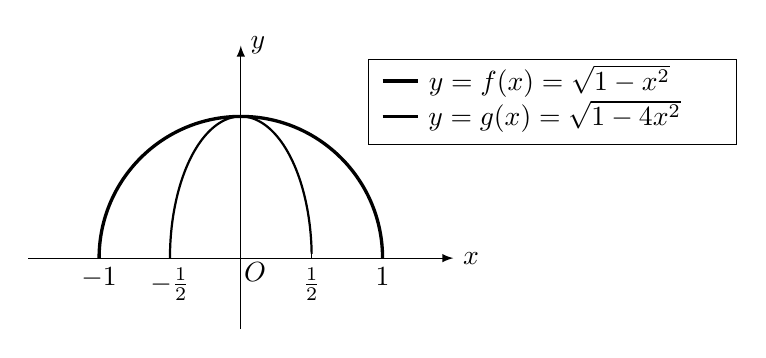
\begin{tikzpicture}[>=latex, scale=1.8]
    \draw[->] (-1.5,0)--(1.5,0)node[right]{$x$};
    \draw[->] (0,-.5)--(0,1.5)node[right]{$y$};
\draw [very thick](-1,0) arc (180:0:1);
\draw[domain=-.5:.5, samples=1000, thick] plot(\x, {sqrt(1-4*\x*\x)});
\foreach \x/\xtext in {-1/-1,-.5/-\frac{1}{2},.5/\frac{1}{2},1/1}
{
    \draw (\x,0)node[below]{$\xtext$}--(\x,.1);
}
\node at (.1,-.1){$O$};
\draw[thick] (1,1)--(1.25,1)node[right]{$y=g(x)=\sqrt{1-4x^2}$};
\draw[very thick] (1,1.25)--(1.25,1.25)node[right]{$y=f(x)=\sqrt{1-x^2}$};
\draw (.9,.8) rectangle (3.5,1.4);
\end{tikzpicture}
    \caption{}\label{fig:function_transform}
\end{figure}
\end{solution}

\begin{ex}
\begin{question}
  \item 试由函数增减性的定义,说明下面函数的增减性:
  \begin{tasks}(2)
    \task $y=x^3$
    \task $y=x^{-2}$
    \task $f(x)=\sqrt{x}$
    \task $g(x)=\sqrt[3]{x}$
    \task $h(x)=\frac{1}{\sqrt{x}}$
  \end{tasks}        
  \item 作下列函数的图象:
  \begin{tasks}(2)   
    \task $y=\sqrt{x}$
    \task $y=x-[x]$
    \task $y=\sqrt{x-[x]}$
    \task $y=[x]+\sqrt{x-[x]}$
  \end{tasks}        
  \item 若一折线函数的图象 $ABCDE$ 的顶点坐标是
  \[A\left(-1,-1\frac{1}{2}\right),\quad B(1,1),\quad C(3,-1),\quad D(6,2.5),\quad E(7,2.5)\]    
写出这个函数的解析式。

\item 作下列函数的图象:
\begin{tasks}(2)  
  \task $f(x)=|2x|$
  \task $f(x)=\dfrac{|x|}{x}$
  \task $y=|4-x^2|,\quad -3\leqslant x\leqslant 3$
  \task $y=|x^2-2x-3|$
\end{tasks}        
\item 已知点 $P(\alpha,\beta)$和一水平线 $L$ 即 $g(x)=\gamma$ 的图象。证明至 $P$ 与 $L$ 等距离的所有点 $(x,y)$ 的集合,是具有 $f(x)=ax^2+bx+c$ 形式的函数的图象。
\end{question}
\end{ex}

\section{函数的连续性}
在初中一年级讨论平方根时,我们曾用下面的想法初步地肯定$\sqrt{2}$的“存在性”:边长是 1 米的正方形面积是 1 平方米;边长是 2 米的正方形面积是 4 平方米,所以,当一个正方形的边长逐渐增加时,它的面积逐渐由 1 平方米增加到 4 平方米,中间应该会有那么一个 2 平方米的正方形。

上面这段话只是一个粗略的想法,用数学语言来表达如下:

$y=f(x)=x^2$,这个幂函数的函数值,在 $x=1$ 时,$f(1)=1^2=1$;$x=2$ 时,$f(2)=2^2=4$;当 $x$ 由 1 变到 2 时,$x$的值应该由 1 “连续地”变到 4,所以 $x$ 应该能取一个值 $x_0$ 使 $f(x_0)=x^2_0=2$。

上面说的“连续地”这个术语究竟是什么意思呢?在这一节中,我们就是要把“连续性”的涵意加以分析、确立。并且,把上面这个粗略的想法体现成一个明确有用的定理——中间值定理。

\subsection{连续函数的概念}
从几何的直观来看,连续与间断的意思是一目了然的,一条曲线是连续的,指这条曲线没有间断点,在上一节考察的函数,展示了函数图象有间断点的情形,函数 $f$ 在点 $x_0$ 是
否连续只依赖于它在 $x_0$ 的一个(任意小的)邻域内的变化情况。直观地看来,如果
\begin{enumerate}
  \item $f$ 在其定义域的点 $x_0$ 的邻域 $(x_0-\delta,x_0+\delta) $内有定义;
  \item 当 $x$ 充分接近 $x_0$ 时,函数值 $f(x)$ 同 $f(x_0)$ 相差任意小,即自变量$x$ 的微小变化只能引起函数值的微小变化,从而排除了函数值的跳跃,就函数的图象来看,在这一点 $x_0$ 的邻近,函数图象是由一条曲线组成的,而没有在这一点断开成为两个分支,那么称函数 $f$ 在点 $x_0$ 连续。
\end{enumerate}

“充分接近”和“相差任意小”这两句话是不够明确的,而必须用定量的术语给以严格的表述。现在我们可以用数列极限的概念把“当 $x$ 充分接近 $x_0$ 时,$f(x)$ 与 $f(x_0)$ 相差任意小”这句话定量地描述如下:

如果在函数定义域 $I$ 中,自变量 $x$ 取任何一个收敛于 $x_0\in I$(即$\displaystyle\lim_{i\to\infty}x_i=x_0$)的数列 $\{x_i\}$ 的项 $x_i\; (i=1,2,\ldots)$,那么对应的函数数列:
\[f(x_1),\; f(x_2),\; \ldots,\;  f(x_i),\ldots\]
总有极限值 $f(x_0)$,即
\[\lim_{i\to\infty} f(x_i)=f(x_0)\]

于是我们得到下述连续性的严格定义:

\begin{Definition}
  定义在区间 $I$ 上的一个函数 $f$ 在点 $a\in I$ 称做连续,如果
\begin{enumerate}
  \item $f(a)$ 有一个确定值,
  \item 对于 $I$ 中每一个收敛于 $a$ 的数列 $\{x_i\}$,对应的函数数列 $\{f(x_i)\}$ 总以 $f(a)$ 为极限,即有关系式:
  $\displaystyle\lim_{i\to \infty}f(x_i)=f(a)=f\left(\lim_{i\to \infty}x_i\right)$
  成立。
\end{enumerate}
\end{Definition}

这个定义表明对于一个连续函数 $f$, 记号 $\lim$ 可以和记号 $f$ 互换。

我们举几个例子说明如何用这个定义来验证函数 $f$ 在点 $a$ 处连续或间断。

\begin{example}\label{exp:uncontinuous1}
  函数 $f(x)=\dfrac{3}{4}\cdot\dfrac{x^2-1}{x-1}$ 在点 $x=1$ 处不连续,因为
$f(1)$ 没有意义。
\end{example}

\begin{example}\label{exp:uncontinuous2}
{\linespread{1.6}\selectfont 函数 $f(x)=[x]$ 在整数点 $n$ 处不连续,因为当 $x=n,\; (n\in\mathbb{Z})$ 时,函数 $f(x)=[x]$ 有确定值 $f(n)=[n]=n$。虽然当 $x$ 取的数列 $\{x_i\}$的值,从$x=n$ 的右边趋于 $n$ 时,有 $\lim\limits_{i\to\infty}f(x_i)=\lim\limits_{i\to\infty}[x_i]=n=f(n)$, 但是当 $x$ 取的数列 $\{x'_n\}$ 从 $x=n$ 的左边趋于 $n$ 时,即当$x'_i$ 满足条件:$n-1\leqslant x'_i <m$,$\lim\limits_{i\to \infty}x'_i=n$ 时,那么\par}
  \[\lim_{i\to \infty}f(x'_i)=\lim_{i\to \infty}[x'_n]=n-1\ne f(n)=n\]
这就是说 $f(x)=[x]$ 的图象是在整数点具有跳跃性间断的曲线。
\end{example}

现在我们来考虑另一种间断性的曲线。
\begin{example}\label{exp:uncontinuous3}
函数 $f(x)=\dfrac{1}{x}$ 在点 $x=0$ 处不连续,因为 $f(0)$ 不存在,并且任何数列 $\{x_i\}$ 收敛于 0 时,例如:

当 $x_i>0$,$x_i\to 0$ 时,即 $x_i$ 从右边趋近于原点时,有 $\lim\limits_{i\to\infty}\dfrac{1}{x_i}=+\infty$;

当 $x_i<0$,$x_i\to 0$ 时,即 $x_i$ 从左边趋近于原点时,有 $\lim\limits_{i\to\infty}\dfrac{1}{x_i}=-\infty$;

当 $\{x_i\}$ 是任意一个趋于0的数列时,则 $\lim\limits_{i\to\infty}\left|\dfrac{1}{x_i}\right|=\infty$。

无论哪种情形,数列 $\left\{\dfrac{1}{x_i}\right\}$ 趋向无穷大。
\end{example}

\begin{rmk}
\cref{exp:uncontinuous1,exp:uncontinuous3} 的分母的零点都是函数的不连续点,
但是\cref{exp:uncontinuous1} 中的分式:$f(x)=\dfrac{3}{4}\cdot\dfrac{x^2-1}{x-1}$,当 $x=1$ 时,代数恒等式
\[\frac{3}{4}\cdot\frac{x^2-1}{x-1}=\frac{3}{4}(x+1)\]
是成立的。因此任何数列 $x_i\; (\ne 1)$ 趋于 1 时,由于 $x_i\ne 1$,
\[\begin{split}
  \lim_{i\to\infty}f(x_i)&=\lim_{i\to\infty}\frac{3}{4}\cdot \frac{x^2_i-1}{x_i-1}=\lim_{i\to\infty}\frac{3}{4}(x_i+1)\\
  &=\frac{3}{4}(1+1)=\frac{3}{2}
\end{split}\]

这就是说,对于任何收敛于1的数列 $\{x_i\}$,对应的函数数列 $\{f(x_i)\}$ 都以$\frac{3}{2}$ 为极限。 

如果我们定义一个新函数 $F$:
\[F(x)=\begin{cases}
    \dfrac{3}{4}\cdot\dfrac{x^2-1}{x-1},& x\ne 1\\
    \dfrac{3}{2}, & x=1
\end{cases}\]
那么 $F(x)$ 在点 $x=1$ 处就连续了。
\end{rmk}

\begin{Definition}
如果对于任何收敛于 $a$ 的数列 $\{x_i\}$, $\lim\limits_{i\to\infty}f(x_i)$ 存在,并且彼此相等,但不等于 $f(a)$,或者 $f(a)$ 没有定义,则称 $f$ 在 $a$ 处有可去间断点。
\end{Definition}

\cref{exp:uncontinuous1} 中的 $x=1$ 就是 $f$ 的可去间断点。

\begin{Definition}
  如果函数 $f$ 在定义域 $I$ 中每一点都连续,就说 $f$ 是 $I$ 上的一个连续函数,或简称为连续函数。
\end{Definition}

\subsection{连续函数的运算}
由连续函数定义知道,函数 $f$ 在 $a\in I$ 连续当且仅当:若 $I$ 里的每个数列 $\{x_i\}$ 收敛于 $a$ 时,数列 $\{f(x_i)\}$ 也收敛于 $f(a)$。

我们可以把上述条件:
\[\lim_{i\to \infty}x_i=a \quad \Longrightarrow\quad \lim_{i\to \infty}f(x_i)=f(a)\]
简写成:
\[\lim_{x\to a}f(x)=f(a)=f\left(\lim_{x\to a}x\right)\]

由数列极限运算定理直接得出下面定理。

\begin{Theorem}{定理1}
  设 $f$ 和 $g$ 在 $a$ 处连续,即
  \[\lim_{x\to a}f(x)=f(a),\qquad \lim_{x\to a}g(x)=g(a)\]
  则
\begin{enumerate}[itemsep=5pt]
    \item $\lim\limits_{x\to a}[f(x)\pm g(x)]=f(a)\pm g(a)$,(即 $f\pm g$ 在$a$ 处连续)。
    \item $\lim\limits_{x\to a}f(x)\cdot g(x)=f(a)\cdot g(a)$,(即 $f\cdot g$ 在 $a$ 处连续)。
    \item 若 $g(a)\ne 0$,$\lim\limits_{x\to a}\dfrac{1}{g(x)}=\dfrac{1}{g(a)}$,(即 $1/g$ 在 $a$ 处连续)。
\end{enumerate}
\end{Theorem}

\begin{example}
  函数 $f(x)=x^k$($k$ 是一个正整数,$x\in\mathbb{R}$)到处连续,即 $\lim_{x\to a}x^k=a^k,\; (a\in\mathbb{R})$。
\end{example}

\begin{proof}
对 $k$ 用数学归纳法来证明,设 $a$ 是 $f$ 的定义域 $\mathbb{R}$ 中任何一点。

当 $k=1$ 时,显然,$\lim_{x\to a}x=a$, 命题成立。

假设当 $k=i\; (i\in\mathbb{N})$ 时,有
\[\lim_{x\to a} x^i=a^i\qquad (i\in\mathbb{N})\]
那么,当 $k=i+1$ 时,有
\[\lim_{x\to a}x^{i+1}=\lim_{x\to a} x^i\cdot x=\lim_{x\to a} x^i\cdot \lim_{x\to a} x=a^i\cdot a=a^{i+1}\]    
于是,对于所有正整数 $k$,$f(x)=x$ 在任何一点 $a$ 连续,也即 $f(x)=x$ 到处连续。
\end{proof}


由定理 1 和 $f(x)=x^k\; (k\in\mathbb{N})$, 及常数函数 $g(x)=c$($c$ 是常数)的到处连续性,我们可以证明下面的命题成立。

\begin{Theorem}{命题1}
  任何多项式函数到处连续。
\end{Theorem}

进一步推得下面命题:

\begin{Theorem}{命题2}
若 $f$ 和 $g$ 是两个多项式,$g\ne 0$,那么有理函数 $r=f/g$,除去 $g$ 的零点集合,函数 $r$ 是有定义的而且是连续的。
\end{Theorem}

\begin{Theorem}{命题3}
  $f(x)=\sqrt[\uproot{3}\leftroot{-1}n]{x}$ 在区间 $(0,+\infty)$ 上连续,即 
\[\lim_{x\to x_0}\sqrt[\uproot{3}\leftroot{-1}n]{x}=\sqrt[\uproot{3}\leftroot{-1}n]{x_0}\qquad (x\in[0,+\infty))\]
\end{Theorem}

\begin{proof}
  设 $x_0$ 是一个任给正数,数列 $\{x_i\}$是在$[0,+\infty)$
内任何一个收敛到 $x_0$ 的数列,即 $\lim\limits_{i\to \infty} x_i=x_0$。我们要证明,当 $\lim\limits_{i\to\infty} x_i=x_0$ 时,$\lim\limits_{i\to\infty} (\sqrt[\uproot{3}\leftroot{-1}n]{x_i}-\sqrt[\uproot{3}\leftroot{-1}n]{x_0})=0$。

\medskip
在代数恒等式:
\[(A-B)\left(A^{n-1}+A^{n-2}B+\cdots +AB^{n-2}+B^{n-1}\right)=A^n-B^n\]
中,以 $A=x_i^{\tfrac{1}{n}}$,$B=x_0^{\tfrac{1}{n}}$ 代入,即得:
\begin{equation}
  \label{eq:subtraction_power}
\sqrt[\uproot{3}\leftroot{-1}n]{x_i}-\sqrt[\uproot{3}\leftroot{-1}n]{x_0}=\frac{x_i-x_0}{x_i^{\tfrac{n-1}{n}}+x^{\tfrac{n-2}{n}}_i\cdot x_0^{\tfrac{1}{n}}+\cdots +x^{\tfrac{1}{n}}_i\cdot x_0^{\tfrac{n-2}{n}} + x_0^{\tfrac{n-1}{n}}} 
\end{equation}
由于 $\lim\limits_{i\to\infty}x_i=x_0$,根据数列极限定义,取
$\varepsilon=\dfrac{x_0}{2}$,则存在正整数 $N$,使得当 $i>N$ 时,有
\[x_i>x_0-\frac{x_0}{2}=\frac{x_0}{2}\]
从而,当 $i>N$ 时,有
\begin{equation}
  \label{eq:xi_vs_x0}
  (x_i)^{\tfrac{1}{n}}=\left(\frac{x_0}{2}\right)^{\tfrac{1}{n}}
\end{equation}
此外,显然有
\begin{equation}
  \label{eq:x0}
  (x_0)^{\tfrac{1}{n}}>\left(\frac{x_0}{2}\right)^{\tfrac{1}{n}}
\end{equation}

由\cref{eq:subtraction_power,eq:xi_vs_x0,eq:x0} 立即得
\[\left|\sqrt[n]{x_i}-\sqrt[n]{x_0}\right|<\frac{|x_i-x_0|}{n\left(\sqrt[\uproot{12}\leftroot{-3}n]{\dfrac{x_0}{2}}\right)^{n-1}}\]
当 $i\to\infty$ 时,$|x_i-x0|\to 0$,又因为 $n\left(\sqrt[\uproot{12}\leftroot{-3}n]{\dfrac{x_0}{2}}\right)^{n-1}$ 是一个和 $i$ 无关的常数,所以
\[\left|\sqrt[\uproot{3}\leftroot{-1}n]{x_i}-\sqrt[\uproot{3}\leftroot{-1}n]{x_0}\right|\to 0\]
即
\[\lim_{x\to x_0} \sqrt[\uproot{3}\leftroot{-1}n]{x}=\sqrt[\uproot{3}\leftroot{-1}n]{x_0}\]
这也就证明了 $f(x)=\sqrt[\uproot{3}\leftroot{-1}n]{x}$ 在区间 $[0,\infty)$ 上到处连续。
\end{proof}

我们在这里介绍了函数连续性的严格定义,对于初学者只要能够正确理解这一分析定义的涵义就可以了,以后在第六册微积分中,我们还要对它进行研究。

\subsection{连续函数的中间值定理}
平面上一个一目了然的性质是:一条直线把平面分割成两半,例如,在 $(x,y)$ 坐标平面上,直线 $y=c$ 就把平面分成 $y<c$ 和 $y>c$ 这两半,从上半平面走到下半平面的连续通路,必须和分界线 $y=c$ 相交,下述中间值定理也就是上述直观现象的代数化:

\subsubsection{中间值定理}

设 $y=f(x)$ 是一个在闭区间 $[a,b]$ 上到处连续的函数,设 $c$ 是一个介于 $f(a)$ 和$f(b)$ 之间的常数,则必存在一个介于 $a,b$ 之间的实数 $x_0$,使得 $f(x_0)=c$。用几何术语来说:$y=f(x)$,$a\leqslant x\leqslant b$ 的图象是一条连结 $P(a,f(a))$ 点和 $Q(b,f(b))$ 点的连续曲线,而 $P,Q$ 分居于直线 $y=c$ 的两侧,则曲线 $y=f(x),\; a\leqslant x\leqslant b$ 至少和直线 $y=c$ 有一个交点 $(x_0,f(x_0)=c)$,(\cref{fig:curve})。

\begin{figure}
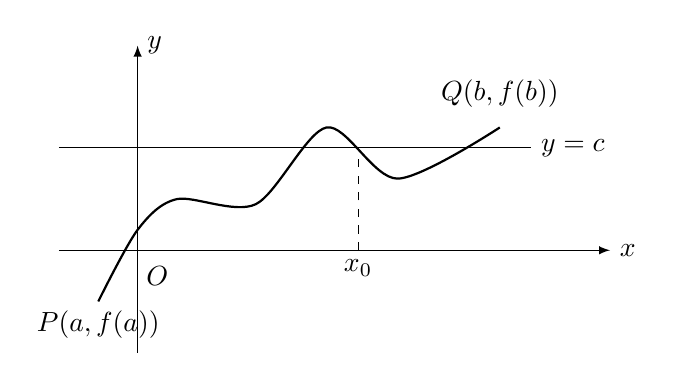
\begin{tikzpicture}[>=latex, yscale=1.3]
    \draw[->] (-1,0)--(6,0)node[right]{$x$};
    \draw[->] (0,-1)--(0,2)node[right]{$y$};
    \draw(-1,1)--(5,1)node[right]{$y=c$};
    \node at (.25,-.25){$O$};
    \draw[ thick] plot[smooth] coordinates{(-.5,-.5)(0,.2) (.5,.5) (1.5,.45) (2.4,1.2)(3.3,.7)(4.6,1.2)};
\node at (-.5,-.5)[below]{$P(a,f(a))$};
\node at (4.6,1.3)[above]{$Q(b,f(b))$};
\draw[dashed] (2.8,0)node[below]{$x_0$}--(2.8,1);
\end{tikzpicture}
    \caption{}\label{fig:curve}
\end{figure}

在给出这个定理的证明之前,我们先讨论一个特例,让 $f(x)=x^3+x-3$, $a=1$, $b=2$。由于 $f(1)=-1$ 与 $f(2)=7$ 异号,我们将说明在 $1,2$ 之间一定存在 $f(x)=x^3+x-3$ 的根 $k$,使 $f(k)=0$。

从 $y=x^3+x-3$ 的图象(\cref{fig:cubic_curve})上看,这个命题是一目了然的,现在我们要把二分逼近法与实数完备性,函数连续性配合一起来说明它的根的存在和根的求法。

\begin{figure}
\begin{tikzpicture}[>=latex, yscale=.6]
\draw[->] (-2,0)--(3,0)node[right]{$x$};
\draw[->] (0,-9)--(0,8)node[right]{$y$};
\foreach \x in {-8,-7,...,-1,1,2,...,7}
{
    \draw (-.1,\x) node[left]{$\x$} --(0,\x);
}
\node at (.4,-.4){$O$};
\draw[domain=-1.6:2, samples=100, very thick] plot(\x, {\x*\x*\x+\x-3});
\node at (2,5)[right]{$y=x^3+x-3$};
\end{tikzpicture}
    \caption{}\label{fig:cubic_curve}
\end{figure}


首先,我们容易验证这个方程没有整数根 $\pm 1$ 和 $\pm 2$,因此所求的根一定是一个无理数,由于闭区间 $[a,b]=[1,2]$ 具有性质 $P:f(a)\cdot f(b)<0$,即 $f(a)$ 与$f(b)$ 异号。当我们把它二等分时,至少会有一个分段保有这个性质 $P$,照这样,不断地二等分保有性质 $P$ 的分段,我们就可以得到保有性质 $P$ 的两串左、右夹逼数列如下:

令 $x=\dfrac{1+2}{2}=\dfrac{3}{2}$,显然 $f\left(\dfrac{3}{2}\right)\ne 0$,否则$f(x)$ 就会有有理数根 $\dfrac{3}{2}$,无论 $f\left(\dfrac{3}{2}\right)$ 是正还是负,在 $\left[1,\dfrac{3}{2}\right]$ 和 $\left[\dfrac{3}{2},2\right]$ 这两个分段中一定有一段具有性质 $P$,算出
\[f\left(\frac{3}{2}\right)=\frac{3}{8}>0\]

取 $a_1=1$,$b_1=\dfrac{3}{2}$,闭区间 $[a_1,b_1]=\left[1,\dfrac{3}{2}\right]$ 保有性质 $P$,照这样进行有限次后,由于 $f(x)$ 没有有理根,所以 $f\left(\dfrac{a_m+b_m}{2}\right)\ne 0$,这就使我们每次由 $[a_m,b_m]$ 选取保有性质 $P$ 的一个分段 $[a_{m+1},b_{m+1}]$ 之后,还可以细分下去,因此,这个过程是无终止的。
\begin{itemize}%[itemsep=10pt]
\item 令 $x=(a_1+b_1)/2=(1+1.5)/2=1.25$,算出 $f(1.125)=0.2031>0$,取 $[a_2,b_2]=[1,1.25]$;
\item 令 $x=(a_2+b_2)/2=(1+1.25)/2=1.125$,算出 $f(1.125)=-0.4512<0$,取 $[a_3,b_3]=\left[1.125,1.25\right]$;
\item 令 $x=(a_3+b_3)/2=(1.125+1.25)/2=1.1875$,算出 $f\left(1.1875\right)=-0.1379<0$,取 $[a_4,b_4]=\left[1.1875,1.25\right]$;
\item 令 $x=(a_4+b_4)/2=(1.1875+1.25)/2=1.2188$,算出 $f\left(1.2188\right)=0.029>0$,取 $[a_5,b_5]=\left[1.1875,1.2188\right]$;
\item 令 $x=(a_5+b_5)/2=(1.1875+1.2188)/2=1.203$,算出 $f\left(1.203\right)=-0.0552<0$,取 $[a_6,b_6]=\left[1.203,1.2188\right]$;
\item 令 $x=(a_6+b_6)/2=(1.203+1.2188)/2=1.211$,算出 $f\left(1.211\right)=-0.0132<0$,取 $[a_7,b_7]=\left[1.211,1.2188\right]$;
\item 令 $x=(a_7+b_7)/2=(1.211+1.2188)/2=1.215$,算出 $f\left(1.215\right)=0.008>0$,取 $[a_8,b_8]=\left[1.211,1.215\right]$;
\item 令 $x=(a_8+b_8)/2=(1.211+1.215)/2=1.213$,算出 $f\left(1.213\right)=-0.0025<0$,取 $[a_9,b_9]=\left[1.213,1.215\right]$;
\end{itemize}

\medskip
这样继续下去,我们得到无穷个闭区间满足下面的条件:
\begin{enumerate}[itemsep=7pt]
    \item $[a,b]=[1,2]\supseteq [a_1,b_1]=\left[1,1.5\right]\supseteq [a_2,b_2]=\left[1,1.25\right]\supseteq [a_3,b_3]=\left[1.1875,1.25\right] 
    \supseteq [a_4,b_4]=\left[1.1875,1.2188\right]\supseteq [a_5,b_5]=\left[1.203,1.2188\right]\supseteq [a_6,b_6]=\left[1.211,1.2188\right]\supseteq [a_7,b_7]=\left[1.211,1.215\right]\supseteq [a_8,b_8]=\left[1.213,1.215\right]\supseteq   \cdots 
    \supseteq  
    [a_n,b_n]=\supseteq\cdots $
    \item $[a_n,b_n]=\dfrac{1}{2}[a_{n-1},b_{n-1}]=\dfrac{1}{2^2}[a_{n-2},b_{n-2}]=\cdots=\dfrac{1}{2^n}[a,b]$
    
    因此,闭区间 $[a_n,b_n]$ 的长 $=\dfrac{1}{2^n}\to 0$。
    \item $f(a_n)<0$,\; $f(b_n)>0$ 恒成立。
\end{enumerate}

\medskip
换言之,得到满足下面性质的夹逼数列$\{a_n\}$, $\{b_n\}$:
\begin{enumerate}[itemsep=5pt]
    \item\label{itm:property_an_bn} $a=1\leqslant a_1=1\leqslant a_2=1\leqslant a_3=1.1875\leqslant a_4=1.1875  \leqslant  a_5=1.203  \leqslant  a_6=1.211  \leqslant  a_7=1.211  \leqslant  a_8=1.213  \le\cdots\leqslant a_n\le\cdots\leqslant b_n\leqslant \cdots \leqslant  b_8=1.215  \leqslant  b_7=1.215  \leqslant  b_6=1.2188  \leqslant  b_5=1.2188   \leqslant  b_4= 1.2188  \leqslant  b_3= 1.25 \leqslant  b_2=1.25  \leqslant  b_1=1.5  \leqslant  b=2$
    
    并且 $(b_n-a_n)=\dfrac{1}{2^n}\to 0$。

\item $f(a_n)<0$,\; $f(b_n)>0$ 恒成立。
\end{enumerate}

\medskip
由 \ref{itm:property_an_bn} 和实数完备性,就得到唯一实数 $k$ 满足
\[a_n\to k\leftarrow b_n,\qquad \text{即}\quad \lim_{n\to\infty} a_n=\lim_{n\to\infty}  b_n=k\]
再由函数 $f(x)=x^3+x-3$ 的到处连续性,即有
\[\lim_{n\to\infty}  f(a_n)=f(k) \qquad  \lim_{n\to\infty}  f(b_n)=f(k)\]
\begin{itemize}
  \item 由 $f(a_n)<0$ 得知 $f(k)\leqslant 0$,
  \item 由 $f(b_n)>0$ 得知 $f(k)\geqslant 0$。
\end{itemize}
所以只有 $f(k)=0$ 才能同时满足上述两种条件。

\medskip
仿照上面的推理,我们得到了连续函数中间值定理的证明如下:

为了叙述方便,我们不妨设 $f(a)<f(b)$。$\big[$当 $f(a)>f(b)$时,我们可以对 $-f(x)$ 和 $-c$ 来作同样的讨论$\big]$。由\cref{fig:curve} 所示,交点可能有好几个,但是我们所要证的是至少有一个交点,我们将用二分法去逼近其中一个交点的坐标 $x_0$。

取 $a_1=a$, $b_1=b$, 把闭区间$[a,b]$二等分。
\begin{itemize}[itemsep=5pt]
  \item 若 $f\left(\dfrac{a_1+b_1}{2}\right)=c$,则就是一个所求的 $x_0$,自然不必再费任何手脚了;
  \item 若 $f\left(\dfrac{a_1+b_1}{2}\right)<c$,则取后半段为 $[a_2,b_2]$;
  \item 若 $f\left(\dfrac{a_1+b_1}{2}\right)>c$,则取前半段为 $[a_2,b_2]$。
\end{itemize}
照这样逐次地由$[a_m,b_m]$去求出它的半段为$[a_{m+1},b_{m+1}]$。因为 $f(a_m)<c$, $f(b_m)>c$, 取 $x_0=\dfrac{a_m+b_m}{2}$
\begin{itemize}[itemsep=5pt]
  \item 若 $f\left(\dfrac{a_m+b_m}{2}\right)<c$ 则取后半段为 $[a_{m+1},b_{m+1}]$;
  \item 若 $f\left(\dfrac{a_m+b_m}{2}\right)>c$ 则取前半段为 $[a_{m+1},b_{m+1}]$;
  \item 若 $f\left(\dfrac{a_m+b_m}{2}\right)=c$ 则 $\dfrac{a_{m}+b_{m}}{2}$ 也就是所求的 $x_0$,而定理得证。
\end{itemize}

\bigskip
总结上述逐步二等分过程,就只有两种可能:一种可能是经过有限次二等分后,有这样的分点 $\dfrac{a_m+b_m}{2}$ 使 $f\left(\dfrac{a_m+b_m}{2}\right)=c$,于是定理得证,另一种可能是没有这样的分点 $\dfrac{a_m+b_m}{2}$ 使 $f\left(\dfrac{a_m+b_m}{2}\right)=c$ 成立,在这种情形下,继续不断二等分,我们得到无限多个退缩闭区间套$[a_n,b_n]$ 满足下列条件:

\begin{enumerate}
  \item\label{itm:condition1} 闭区间的端点形成夹逼数列 $\{a_n\}$, $\{b_n\}$,适合
    \[a_1\leqslant a_2\leqslant \cdots\leqslant a_n\leqslant \cdots \leqslant b_n\leqslant \cdots\leqslant b_2\leqslant b_1\]
并且 $(b_n-a_n)\to 0$。
  \item $f(a_n)<c$, $f(b_n)>c$ 恒成立。
\end{enumerate}

    由条件 \ref{itm:condition1} 和实数完备性就得到唯一实数 $x_0$
    \[\lim_{n\to\infty} a_n=\lim_{n\to\infty} b_n=x_0\quad \text{即}\quad a_n\to x\leftarrow b_n\]
    再由函数 $f(x)$ 在 $x_0$ 连续性即有
\[    \lim_{n\to\infty} f(a_n) = f(x_0),\qquad \lim_{n\to\infty} f(b_n)=f(x_0)\]

由 $f(a_n)<c$,得知它的极限值 $f(x_0)\leqslant c$,同样地,由 $f(b_n)>c$,得知它的极限值 $f(x_0)\geqslant c$。

所以,只有 $f(x_0)=c$ 才能同时满足上述两个条件,定理得证。

\begin{Theorem}{命题1}
  当 $a>0$ 时,$f(x)=x^n-a=0$存在唯一的正实数根,叫做 $a$ 的 $n$ 次算术方根,用符号 $\sqrt[\uproot{3}\leftroot{-1}n]{a}$ 表示。
\end{Theorem}

\begin{proof}
先证存在性。$f(0)=-a<0$, 而
\[f(1+a)=(1+a)^n-a>0\]
所以,由中间值定理 $f(x)=x^n-a$ 在 0 和 $(1+a)$ 之间至少有一个根 $x_0$,使得$f(x_0)=x_0^n-a=0$ 成立。

再证唯一性。因在 $x>0$ 时,$x$ 愈大则它的 $n$ 次方幂 $x^n$ 也愈大,所以 $f(x)$ 在 $x>0$ 时是严格递增的,当然不可能有两个不同的正实数满足 $f(x)=0$。
\end{proof}

上面的命题给常用的“$n$ 次方根函数 $y=\sqrt[\uproot{3}\leftroot{-1}n]{x},\; x\geqslant 0$”提供了理论基础。为了进一步把中间值定理应用到一般的多项式函数上,我们给出下面的命题。

\begin{Theorem}{命题2 }
对于实系数的多项式
$f(x)=a_0x^n+a_1x^{n-1}+\cdots+a_n,\quad (a_0\ne 0)$, 总可以求出一个正数 $P$, 使得当 $x>P$ 时,$f(x)$ 的值与 $a_0x^n$ 的值有相同的符号。
\end{Theorem}

\begin{proof}
$f(x)=x^n[a_0+\varphi(x)]$, 这里 $\varphi(x)=\dfrac{a_1}{x}+\dfrac{a_2}{x^2}+\cdots+\dfrac{a_n}{x^n},\; (x\ne 0)$ 是一个 $\dfrac{1}{x}$ 的实系数多项式。显然,
\[\lim_{x\to\infty} \varphi(x)=0\]
这也就是说,对于给定的 $\varepsilon=|a_0|$,存在一个正数 $P$,使得
当 $x>P$ 时,从而 $0<\dfrac{1}{x}<\dfrac{1}{P}$ 时,有
\[|\varphi(x)|<|a_0|\]
于是 $a_0+\varphi(x)$,$(x>P)$ 与 $a_0$ 同号,因此 $f(x)$ 与 $a_0x^n$ 同号。
\end{proof}

但是要具体地求出 $P$ 的值,还得用一些技巧。令 $g=\max(|a_1|,|a_2|,\ldots,|a_n|)$, 并且先设 $x>P>1$,于是 $0<\dfrac{1}{x}<\dfrac{1}{P}<1$, 从而
\[\begin{split}
    |\varphi(x)|&=\left|\frac{a_1}{x}+\frac{a_2}{x^2}+\cdots+\frac{a_n}{x^n}\right|\\
    &\leqslant g\left(\frac{1}{x}+\frac{1}{x^2}+\cdots+\frac{1}{x^n}\right)< g\cdot \frac{\dfrac{1}{x}}{1-\dfrac{1}{x}}
\end{split}\]
要使
\[|\varphi(x)|<g\cdot \frac{\dfrac{1}{x}}{1-\dfrac{1}{x}}<|a_0|\]
只须 $\dfrac{1}{x}<\dfrac{|a_0|}{g+|a_0|}$,即 $x>1+\dfrac{g}{|a_0|}$。

\medskip
取 $P=1+\dfrac{g}{|a_0|}$,因此,当 $x>1+\dfrac{g}{|a_0|}$ 时,就可以使 $f(x)$ 与$a_0x^n$ 有相同符号。

如果令 $x=-X\; (X>0)$, 前面的情形说明当 $X$ 是一个充分大的正数时,$f(-X)$ 的值的符号就与 $(-1)^na_0X^n$ 的值有相同符号。因此我们得到下面的推论:
\begin{Deduction}{推论}
    对于实系数多项式 $f(x)=a_0x^n+a_1x^{n-1}+\cdots+a^n\; (a_0\ne 0)$
\begin{itemize}
    \item 当 $x$ 充分大时,$f(x)$与$a_0$同号;
    \item 当 $x$ 取负值而 $|x|$ 充分大时,若 $n$ 是偶数,则 $f(x)$ 与 $a_0$ 同
号;若 $n$ 是奇数,则 $f(x)$ 与 $a_0$ 异号。
\end{itemize}
\end{Deduction}

由上面的推论直接得到下面的命题:
\begin{Theorem}{命题 3}
  若 $n$ 为奇数,则实系数方程 $x^n+a_1x^{n-1}+a_2x^{n-2}+\cdots+a_0=0$ 有一个根。 
\end{Theorem}

\begin{Exercise}
\begin{question}[itemsep=5pt]
  \item 证明下列各函数是到处连续的函数:
  \begin{tasks}(2)
      \task $f(x)=|x|$
      \task $g(x)=\frac{x^2}{1+x^2}$
      \task $h(x)=x|x|-\frac{1}{2}$
      \task $\varphi(x)=\sqrt{x}$
  \end{tasks}
  \item 设函数$f(x)=\dfrac{x^2+1}{2x-1}$,则 $f(0)=-1$,$f(1)=2$ 符号相反,讨论方程式 $f(x)=0$ 在 $0\leqslant x\leqslant 1$ 中是否有解?
  \item 下列函数各在哪些点不连续:
  \begin{tasks}(2)
    \task $\displaystyle f(x)=\frac{x+2}{x^2-1}$
    \task $\displaystyle f(x)=\frac{x-1}{(x^2+1)(2x+3)}$
    \task $\displaystyle g(x)=\sqrt{\frac{x-2}{x^2-4}}$
    \task $\displaystyle h(x)=\frac{2}{|x|-1}$
    \task $\displaystyle \varphi(x)=\frac{|x|-1}{|x-1|-4}$
    \task $\displaystyle F(x)=\frac{1}{x-[x]}$
  \end{tasks}
  \item 试证下列多项式有唯一的正实根。
  \begin{tasks}(2)
    \task $x^3+x^2-1=0$;
    \task $x^3-3x^2+3x-4=0$.
  \end{tasks}
  \item 证明 $8x^3-4x^2-18x+9=0$的一根在 0 和 1 之间,一根在 1 和 2 之间,一根在$-2$ 和 $-1$ 之间。
  \item 对于下列各多项式函数 $f$, 求一整数 $n$ 使在 $n$ 和 $n+1$ 之间的某一 $x$ 满足 $f(x)=0$:
  \begin{tasks}(2)
    \task $f(x)=x^3-x+3$;
    \task $f(x)=x^5+x+1$.
  \end{tasks}
  \item 设 $f(x),g(x)$ 是两个连续函数而且 $f(a)>g(a)$,$f(b)<g(b)$, 求证在 $a,b$ 之间存在一个适当 $x_0$,使得 $f(x_0)=g(x_0)$。
  \item 设 $a<b<c$, 证明方程 $\dfrac{1}{x-a}+\dfrac{1}{x-b}+\dfrac{1}{x-c}=2$ 有三个实根,且一个根在 $a,b$ 之间,另一个根在 $b,c$之间。
  \item 用二分逼近法求 $x^3+2x-7=0$ 的正根,使得误差小于 0.01。
\end{question}
\end{Exercise}


\section{反函数和它的图象}

在研究一个问题的时候,不只是把两个变量之间的函数关系表示成 $y$ 是 $x$ 的函数,有时也需要把 $x$ 表示为 $y$ 的函数,例如,在自由落体运动中,如果想从已知的时间 $t$ 来确定路程 $s$,则 $s$ 是 $t$ 的函数
\begin{equation}
  \label{eq:falling}
  s=\frac{1}{2}gt^2
\end{equation}
如果反过来,想从已知的路程 $s$ 来确定下落的时间 $t$,则应从\cref{eq:falling} 将$t$ 解出:
\begin{equation}
    t=\sqrt{\frac{2s}{g}}
\end{equation}
这时,$t$ 是 $s$ 的函数。

从这里看出,这两个函数 $s=f(t)=\dfrac{1}{2}gt^2$ 和 $t=g(s)=\sqrt{\dfrac{2s}{g}}$,其实是同一种关系的两种表示法,我们把这样的两个函数 $f$ 和 $g$ 叫做互为反函数。

\begin{example}
  若 $x\in\mathbb{R}$, $y\in\mathbb{R}$, 那么,函数
\[f:\; y=f(x)=2x+3,\qquad g:\; x=g(y)=\frac{y-3}{2}\]
互为反函数。
\end{example}


\begin{example}
 若 $x\in X=\{x|0\leqslant x\leqslant 1\}$, $y\in Y=\{y|0\leqslant y\leqslant 1\}$,而 $x,y$ 之间的关系是 $x^2+y^2=1$, 则函数
\[\begin{split}
  f:\; y&=f(x)=\sqrt{1-x^2}\\
g:\; x&=g(y)=\sqrt{1-y^2}   
\end{split}\]
互为反函数,因为在上述关系 $x^2+y^2=1$ 中,$x,y$ 是对称的,所以 $f$ 和 $g$ 是同一形式的函数。在一般情况下 $f$ 和 $g$ 是不同形式的函数。
\end{example}

必须注意,不能认为从每一个函数 $y=f(x)$ 都能解得一个反函数 $x=g(y)$。例如,如果两个变数 $x,y$ 之间的关系是$y=x$, 定义域 $X=\{x|x\in\mathbb{R}\}$, 值域 $Y=\{y|y\geqslant 0\}$,那么:
$f:\; y=x,\; x\in (-\infty,+\infty)$ 是 $X\mapsto Y$ 的函数。但是,如果不对自变数 $x$ 加以限制,这个函数 $f$ 是不可逆的,也就是由它不能得到一个新函数 $g:\; Y\mapsto X$。因为,对于每个 $y(\ne 0)\in Y$, 将有 $X$ 中两个数值 $x=\sqrt{\mathstrut y}$ 和$x=-\sqrt{\mathstrut y}$ 和 $y$ 对应,如\cref{fig:mapping} 所示:

\begin{figure}
    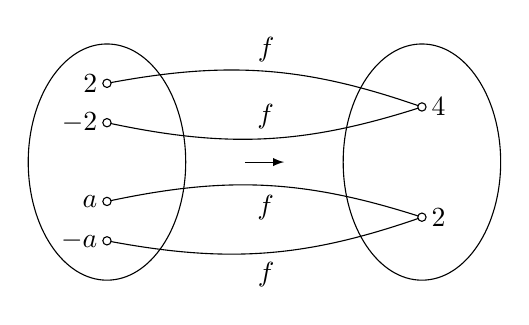
\begin{tikzpicture}[>=latex]
\draw (0,0) ellipse [x radius=1, y radius=1.5];
\draw (4,0) ellipse [x radius=1 ,y radius=1.5];

\draw(0,1)to [bend left=15] node[above]{$f$} (4,.7);
\draw (0,.5)to [bend left=-15]node[above]{$f$} (4,.7);
\draw (0,-1)to [bend left=-15]node[below]{$f$}(4,-.7);
\draw (0,-.5)to [bend left=15]node[below]{$f$} (4,-.7);

\draw[->](1.75,0)--(2.25,0);

\foreach \x/\xtext in {1/2,.5/-2,-.5/a,-1/-a}
{
    \draw (0,\x) [fill=white]circle (1.5pt)node[left]{$\xtext$};
}
\foreach \x/\xtext in {.7/4,-.7/2}
{
    \draw (4,\x) [fill=white]circle (1.5pt)node[right]{$\xtext$};
}
    \end{tikzpicture}
    \caption{}\label{fig:mapping}
\end{figure}


下面我们来说明具有怎样性质的函数才有反函数。

假如函数 $y=f(x)$ 具有这样的性质:“若 $x_1\ne x_2\; \Rightarrow\; f(x_1)\ne f(x_2)$,也就是说对于定义域 $X$ 中任意不同的 $x_1$, $x_2$,它们在值域 $Y=f(X)$ 中的对应值$f(x_1)$, $f(x_2)$也不相同”。那么对于 $Y=f(X)$ 内任何一个 $y$,通过函数 $f$,可以逆对应出一个且只有一个 $x$,使得 $y$ 和这个 $x$ 对应,这样一个函数叫做由 $X$ 到 $Y=f(X)$ 的一一对应函数,或双射(满射且单射),简称这个函数是\emph{可逆}的。对于一个可逆函数 $f:\; x\mapsto f(x)$,我们可以交换自变数与因变数的地位,于是对于 $Y=f(X)$ 的每一个 $y$ 就有 $X$ 内唯一一个逆象 $x$,这就是说我们得到了一个新函数:
\[ g:\; Y=f(X)\mapsto X,\qquad \text{使得}\; y\mapsto x=g(y)\]
假如 $y=f(x)$。

新函数和原来函数的这种关系可以用下图来说明:
\begin{center}
  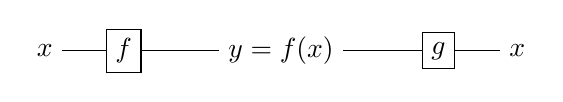
\begin{tikzpicture}
      \node (A) at (1,0) {$x$};
      \node[rectangle, draw] (B) at (2,0) {$f$};
      \node (C) at (4,0) {$y=f(x)$};
      \node[rectangle, draw] (D) at (6,0) {$g$};
      \node (E) at (7,0) {$x$};    
      \draw (A)--(B)--(C)--(D)--(E);
  \end{tikzpicture}
\end{center}

根据上面的分析,我们得到反函数的一般定义如下:
 
\begin{Definition}
  设给了一个函数 $y=f(x)$,其定义域为 $X$,值域为 $Y=f(X)$,如果对于 $Y=f(X)$ 中每一个 $y$ 值,都可以从关系式 $y=f(x)$ 确定唯一的一个 $x$ 值,则得到一个定义在 $Y=f(X)$ 上而且把 $f(X)=Y$ 映射到 $X$ 上的以 $y$ 为自变数的新函数 $x=g(y)$,这个函数称为函数 $y=f(x)$ 的反函数。
\end{Definition}

不难理解 $f$ 也是 $g$ 的反函数,并且函数 $y=f(x)$ 与它的反函数 $x=g(y)$ 组成的复合函数一定是一个恒等函数,即 
\[ g\big(f(x)\big)=x,\qquad f\big(g(y)\big)= y\]
有时用符号 $f^{-1}$ 表示反函数比较方便,如
\[f^{-1}\big(f(x)\big)=x,\qquad f\big(f^{-1}(y)\big)=y\]

按照函数 $y=f(x)$ 的图象容易判断函数 $y=f(x)$ 是否有反函数存在,就是在值域 $Y=f(X)$ 内,任意给一个值 $y_0$,作和 $x$ 轴平行的直线 $y=y_0$。如果函数$y=f(x),\; x\in X$ 的图象和直线 $y=y_0$ 的交点多于一个,那么这个函数的反函数就
不存在。如果只有一个交点,那么这个函数就有反函数。如\cref{fig:inverse_function} 所示。

\begin{figure}
    \begin{tikzpicture}[>=latex]
\begin{scope}
    \draw[->] (-2,0)--(4,0)node[right]{$x$};
        \draw[->] (0,-1)--(0,2)node[right]{$y$};
        \draw(-2,1)--(3,1)node[right]{$y=y_0$};
        \node at (-.25,-.25){$O$};
        \draw[ thick] plot[smooth] coordinates{(-1.7,-.5)(-1.0,.6)(0,1.2) (1.2,-.3)(1.6,-.5)(2,-.3) (2.5,1.2) };
    \node at (2.5,1.2)[above]{$y=f(x)$是不可逆的};
\end{scope}
\begin{scope}[xshift=7.5cm]
    \draw[->] (-2,0)--(4,0)node[right]{$x$};
    \draw[->] (0,-1)--(0,2)node[right]{$y$};
    \draw(-2,1)--(3,1)node[right]{$y=y_0$};
    \node at (-.25,-.25){$O$};
    \draw[ thick] plot[smooth] coordinates{(-1.5,-.5)(-.7,.3) (0,.5) (1.3,.7) (2.5,1.8)};
    \node at (2.5,1.8)[above]{$y=f(x)$ 是可逆的};
\end{scope}        
    \end{tikzpicture}
    \caption{}\label{fig:inverse_function}
\end{figure}

{\linespread{1.6}\selectfont 现在我们来研究互为反函数的图象的关系,因为互为反函数的两个函数 $y=f(x)$ 和$x=g(y)$ 事实上就是同一个关系,在几何上就是同一条曲线。例如函数 $y=2x+3$ 的图象和它的反函数 $x=\dfrac{1}{2}(y-3)$ 的图象就是通过两个点 $\left(-\dfrac{3}{2},0\right)$, $(0,3)$ 的同一条直线 $2x-y+3=0$,只是就函数 $y=f(x)=2x+3$ 的图象去看,横轴是自变量轴,而就反函数 $x=g(y)=\dfrac{1}{2}(y-3)$ 的图象来看,纵轴是自变量轴,但是在同一个坐标系内,一般我们总规定用横坐标 $x$ 表示自变数,纵坐标 $y$ 表示因变数,所以我们还需要把反函数关系式 $x=g(y)$ 的 $x,y$ 对调一下,得到习惯上的反函数 $y=g(x)$。我们也称 $y=g(x)$ 是 $y=f(x)$ 的反函数,当然反过来 $y=f(x)$ 也是 $y=g(x)$ 的反函数,例如函数 $y=2x+3$ 和 $y=\dfrac{1}{2}(x-3)$ 互为反函数。\par}

\medskip
函数 $y=f(x)$ 和它的反函数$y=f^{-1}(x)$ 的图象之间有如下关系:

若点 $(a,b)$ 在曲线 $y=f(x)$ 上,那么点 $(b,a)$ 就在曲线 $y=f^{-1}(x)$ 上。

事实上,因为点 $(a,b)$ 在曲线 $y=f(x)$ 上,所以 $b=f(a)$ 成立,此等式也可以写成$a=f^{-1}(b)$,这表示点 $(b,a)$ 在曲线 $y=f^{-1}(x)$ 上,于是当点 $(a,b)$ 走遍曲线 $y=f(x)$ 时,点 $(b,a)$ 就走遍曲线 $y=f^{-1}(x)$。通过初等几何的方法可以证明点 $(a,b)$ 和 $(b,a)$ 关于第一象限角和第三象限角的平分线 $y=x$ 对称。因此,为了得到反函数 $y=f^{-1}(x)$ 的图象,我们只要把 $y=f(x)$ 的图象关于直线 $y=x$ 反射过来就可以。如\cref{fig:inverse_func_graph} 所示。
\begin{figure}
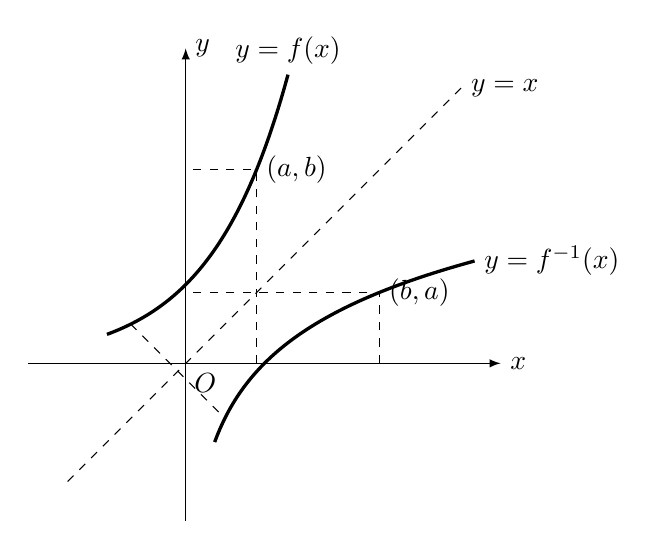
\begin{tikzpicture}[>=latex]
    \draw[->] (-2,0)--(4,0)node[right]{$x$};
    \draw[->] (0,-2)--(0,4)node[right]{$y$};
    \draw [domain=-1:1.3, samples=100,  very thick]plot(\x, {exp(\x)});
    \draw [domain=exp(-1):exp(1.3), samples=100,  very thick]plot(\x, {ln(\x)});
\draw[dashed] (-1.5,-1.5)--(3.5,3.5)node[right]{$y=x$};
\draw[dashed] (2.46,0)--(2.46,.9)node[right]{$(b,a)$}--(0,.9);
\draw[dashed] (.9,0)--(.9,2.46)node[right]{$(a,b)$}--(0,2.46);
\draw[dashed]  (-.7,.5)--(.5,-.7);
\node at (.25,-.25){$O$};
\node at (3.67,1.3)[right]{$y=f^{-1}(x)$};
\node at (1.3,3.67)[above]{$y=f(x)$};
\end{tikzpicture}
    \caption{}\label{fig:inverse_func_graph}
\end{figure}

最后,我们给出一个反函数定理:

\begin{Theorem}{定理}
设 $y=f(x)$ 在闭区间 $[a,b]$ 上严格递增(递减)且连续,又 $f(a)=\alpha$,$f(b)=\beta$,则在闭区间 $[\alpha,\beta]$ 上存在着 $y=f(x)$ 的反函数 $x=f^{-1}(y)$,又 $x=f^{-1}(y)$ 在 $[\alpha,\beta]$(或 $[\beta,\alpha]$)上也是严格递增(或递减)且连续的。
\end{Theorem}

\begin{proof}
\begin{enumerate}
\item 先证 $y=f(x)$ 的值域是闭区间 $[\alpha,\beta]$,设 $y$ 是 $[\alpha,\beta]$ 中任意一点,如果 $y=\alpha$ 或 $\beta$,那么相应的 $x=a$ 或 $b$,即有 $f(a)=\alpha$ 或 $f(b)=\beta$,换言之,$\alpha ,\beta$ 在 $f(x)$ 的值域中。又如果 $\alpha=f(a)<y_0<f(b)=\beta$,由连续函数中间值定理,在$[a,b]$ 之间必存在一点 $x_0$ 满足 $f(x_0)=y_0$,即$[\alpha ,\beta]$  内任一点都属于值域 $f([a,b])$,又如果 $y_0\notin [\alpha ,\beta]$,那么由严格递增性得出,它不可能是任一点 $x\in [a,b]$ 的象,这就证明了 $f(x)$ 的值域是 $[\alpha,\beta]$,因此,连续递增函数 $f:[a,b]\mapsto [\alpha ,\beta]$ 是满射的。

\item 再证 $f$ 是单射的,因为一个严格递增函数 $f$ 满足条件
\[x_1<x_2\quad \Rightarrow\quad f(x_1)<f(x_2)\] 
即自变数的值与函数值是一对一的,所以 $f$ 是单射的。

由上可知函数 $f$ 是可逆的,因此存在一个反函数 $f^{-1}:[\alpha,\beta]\mapsto [a,b]$,其中$x=f^{-1}(y)$。
\item 证明 $f^{-1}$ 的递增性。

假设 $y_1,y_2$ 是 $[\alpha,\beta]$ 内的两个数,并且 $y_1<y_2$,又设 $x=f^{-1}(y_1)$,$x_2=f^{-1}(y_2)$,对于这两数 $x_1$ 和 $x_2$ 只有三种可能:
$x_1<x_2$,$x_1=x_2$,$x_1>x_2$。

如果 $x_1\geqslant x_2$,由于 $f$ 的递增性质,知道
\[y_1=f(x_1)\geqslant f(x_2)=y_2\]
这与 $y_1<y_2$ 的假设矛盾,因此,$x_1<x_2$, 即
\[y_1<y_2 \quad \Rightarrow\quad f^{-1}(y_1)=x_1<x_2=f^{-1}(y_2)\]
这就证明了 $x=f^{-1}(y)$ 是 $[\alpha,\beta]$ 上的递增函数。
\item 最后还应证明 $x=f^{-1}(y)$ 在 $[\alpha,\beta]$ 上连续,但是在高中阶段,我们不深究,同学只要知道结论就可以了。
\end{enumerate}    
\end{proof} 


一般来说,一个函数可以分成分段单调的几支,对于每一支得一反函数。

例如,函数 $y=f(x)=x^2,\; x\in\mathbb{R}$ 在区间 $[0,+\infty)$ 或 $(-\infty,0]$ 上连续和严格单调。因为 $[0,b]\subset [0,+\infty)$ 和 $[-b,0]\subset (-\infty,0] $,这个 $b$ 是任意大的正数,因此 $y=x^2,\; x\in\mathbb{R}$ 的两个分段 $y=f_1(x)=x^2,\; x\in [0,b]$ 和 $y=f_2(x)=x^2,\; x\in[-b,0)$ 根据反函数存在定理,分别有反函数:
\[\begin{split}
    x&=f^{-1}_1(y)=\sqrt{y},\qquad y\in [0,b^2]\\    
    x&=f^{-1}_2(y)=-\sqrt{y},\qquad y\in [0,b^2]\\
\end{split}\]
但是当 $b\to+\infty$时,$b^2\to+\infty$,所以,
\begin{itemize}
  \item 连续和递增的一段 $y=f_1(x)=x^2,\; x\in[0,+\infty)$ 的反函
数是 $x=f_1^{-1}(y)=\sqrt{y},\; y\in [0,+\infty)$, 它是连续的和严格
递增的;
\item 连续和递减的一段 $y=f_2(x)=x^2,\; x\in(-\infty,0]$ 的反函数
是 $x=f_2^{-1}(y)=-\sqrt{y},\; y\in[0,+\infty)$,它是连续的和严格
递减的。
\end{itemize}

将 $f_1^{-1}$ 和 $f_2^{-1}$ 中的 $x$ 和 $y$ 对调后,便得到 $f_1$ 和 $f_2$ 的矫形的反函数,(见\cref{fig:inverse_func_parabolic} )。
\[\begin{split}
    y&=f^{-1}_1(x)=\sqrt{x},\qquad y\in [0,+\infty)\\    
    y&=f^{-1}_2(x)=-\sqrt{x},\qquad y\in [0,+\infty)\\
\end{split}\]
\begin{figure}
  \begin{minipage}{0.48\linewidth}\centering
    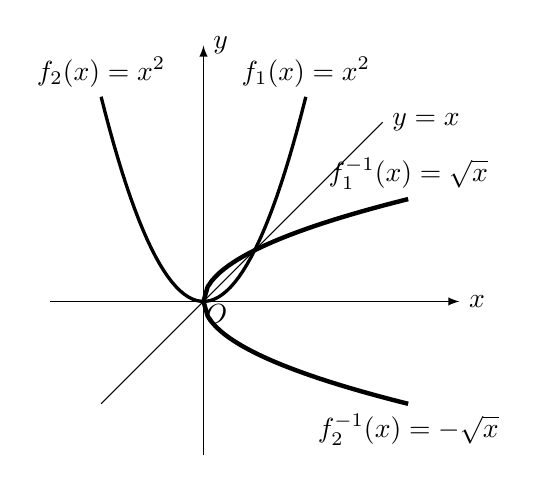
\begin{tikzpicture}[>=latex, scale=.65]
      \draw[->] (-3,0)--(5,0)node[right]{$x$};
      \draw[->] (0,-3)--(0,5)node[right]{$y$};
      \node at (.25,-.25){$O$};
      \draw [domain=-2:2, samples=50, very thick]plot(\x, {\x*\x});
      \draw [domain=0:4, samples=50,ultra thick]plot(\x, {sqrt(\x)});
      \draw [domain=0:4, samples=50,ultra thick]plot(\x, {-sqrt(\x)});
      \draw (-2,-2)--(3.5,3.5)node[right]{$y=x$};
      \node at (-2,4)[above]{$f_2(x)=x^2$};
      \node at (2,4)[above]{$f_1(x)=x^2$};
      \node at (4,-2)[below]{$f_2^{-1}(x)=-\sqrt{x}$};
      \node at (4,2)[above]{$f_1^{-1}(x)=\sqrt{x}$};
    \end{tikzpicture}    
    \caption{}\label{fig:inverse_func_parabolic}
  \end{minipage}
  \begin{minipage}{0.48\linewidth}\centering
    \begin{tikzpicture}[>=latex, scale=1.4]
      \draw[->] (0,0)--(3.5,0)node[right]{$x$};
      \draw[->] (0,0)--(0,3.5)node[right]{$y$};
      \draw [domain=0:1.8, samples=100, thick] plot (\x, {\x^2});
      \draw [domain=0:1.5, samples=100, very thick] plot (\x, {\x^3});
      \draw [domain=0:1.35, samples=100, ultra thick] plot (\x, {\x^4});
      \draw [domain=0:3, samples=100, semithick] plot (\x, {\x});
      \draw [domain=0:3.25, samples=100, thick] plot (\x, {\x^(1/2)});
      \draw [domain=0:3.25, samples=100, very thick] plot (\x, {\x^(1/3)});
      \draw [domain=0:3.25, samples=100, ultra thick] plot (\x, {\x^(1/4)});
      \foreach \x in {1,2,3}
      {
          \draw (\x,0)node[below]{$\x$}--(\x,.05);
          \draw(0,\x)node[left]{$\x$}--(.05,\x);
      }
      \node at (-.1,-.1){$O$};
      \node at (3,3)[right]{$y=x$};
      \node at (1.2,.9){$(1,1)$};
      \node at (1.8,{1.8^2})[right]{$y=x^2$};
      \node at (1.5,{1.5^3})[above]{$y=x^3$};
      \node at (1.35,{1.35^4})[left]{$y=x^4$};
      \node at (3.25,{3.25^(1/2)})[above]{$y=x^{\tfrac{1}{2}}$};
      \node at (3.25,{3.25^(1/3)})[right]{$y=x^{\tfrac{1}{3}}$};
      \node at (3.25,{3.25^(1/4)})[below]{$y=x^{\tfrac{1}{4}}$};
    \end{tikzpicture}
    \caption{}\label{fig:inverse_func_power}
  \end{minipage}
\end{figure}

一般地,函数 $y=f(x)=x^n,\; (n\in\mathbb{N})$ 在半开区间 $[0,+\infty)$ 上
连续和严格递增,函数 $f$ 有反函数
\[x=f^{-1}(y)=\sqrt[n]{y}=y^{\tfrac{1}{n}},\qquad y\in [0,+\infty)\]
它是连续的和严格递增的。

在\cref{fig:inverse_func_power} 中,我们画出几个幂函数和它们的反函数的
图象。

\begin{Exercise}
\begin{question}[itemsep=20pt]
  \item 下列函数在哪些范围内是严格单调的?
  \begin{tasks}(2)
    \task $f(x)=x^3$
    \task $\varphi(x)=x^4$
    \task $y=\sqrt{x}$
    \task $y=\sqrt[3]{x}$
    \task $f(x)=|x+1|$
  \end{tasks}  
  \item 对于下列各函数分别找出它们的最大定义域和值域使得它们有反函数,并分别写出它们的变数 $x$ 表出的反函数。
  \begin{tasks}(2)
    \task $y=\sqrt{2x+1}$
    \task $y=x^{\tfrac{3}{2}}$
    \task $y=x^2-1$
    \task $y=\sqrt{1-x^2}$
    \task $f(x)=\dfrac{x}{1-x^2},\quad -1<x<1$
  \end{tasks}  
  \item 作出下列各函数和它的反函数的图象:
  \begin{tasks}(2)
    \task $y=x^{\tfrac{1}{2}}\quad (x\geqslant 0)$
    \task $y=\dfrac{x+1}{x}\quad (x\ne 0)$
    \task $y=\dfrac{x}{x+1}\quad (x\ne -1)$
  \end{tasks}  
  \item 证明,当且仅当 $ad-bc\ne 0$ 时,$f(x)=\dfrac{ax+b}{cx+d},\; \left(x\ne -\dfrac{d}{c}\right)$ 是单射的,并求它的反函数。又在什么条件下,$f(x)$ 的反函数等于原来函数。
  \item 
  \begin{tasks}
    \task 求 $f(x)=\dfrac{2x-5}{x-3}$ 的反函数 $f^{-1}(x)$。
    \task 已知函数 $f(x)=\dfrac{2x-5}{x-3}$ 的值域是 $\{f(x)|f(x)\leqslant 0,\; f(x)\geqslant 4\}$, 求 $f(x)$ 的定义域。
    \task 设函数 $g(x)=\dfrac{ax-4}{x+b}$ 的反函数是 $g^{-1}(x)=\dfrac{3x+c}{-x+2}$,求实数 $a,b,c$ 的值。
  \end{tasks}
  \item $f(x)=\begin{cases} -x,& x\geqslant 0\\ x^2& x<0 \end{cases}$ 给出由实数集 $\mathbb{R}$ 到 $\mathbb{R}$ 的一个函数 $f$。
  \begin{tasks}
      \task 设 $q(x)$ 是 $f$ 和 $f$ 的复合函数,用 $x$ 的式子表示 $q(x)$。
      \task 设 $q(x)$ 的反函数是 $q^{-1}(x)$,用 $x$ 的式子表示 $q^{-1}(x)$。
  \end{tasks}
\end{question}
\end{Exercise}
